\begin{document}
\frontmatter
\title{Glimmer-CISM {\glimmerver} Documentation}
\author{
\textbf{SP: This author list needs to be updated or made generic}
%Felix Hebeler\thanks{fhebeler@geo.unizh.ch},
%Magnus Hagdorn\thanks{Magnus.Hagdorn@ed.ac.uk}, 
%Tony Payne\thanks{A.J.Payne@bristol.ac.uk},
%Ian  Rutt\thanks{I.C.Rutt@bristol.ac.uk}, 
%and Timothy R. Wylie,
}
\maketitle
\tableofcontents

\ifthenelse{\boolean{html}}
{
\Configure{graphics*} 
         {eps} 
         {\Needs{"convert \csname Gin@base\endcsname.eps 
                               \csname Gin@base\endcsname.png"}% 
          \Picture[pict]{\csname Gin@base\endcsname.png}% 
         } 

}
{}

\mainmatter
\part{User Documentation}

\chapter{User Guide}
\newcommand{\dir}{ug}
%% NOTE: this is the OLD documentation - most of these sections have been replaced with new equivalents
\label{ch:runcism}

\section{Overview of Running CISM}

Assuming you successfully completed the Installation instructions in Chapter \ref{chp:install},
the executable for running the model, \texttt{cism\_driver}, can be found in your 
build directory in a subdirectory called \texttt{cism\_driver} 
(e.g., \texttt{./builds/mac-gnu/cism\_driver/cism\_driver}).

The build system creates the executable at this path but does not automatically
make it available to other locations on your system.  How you choose to do so depends 
on your situation.  See the introduction to Chapter \ref{chp:testcases} for 
an overview of how to make the executable available to other locations on your system
(e.g., symlinking, copying, or modifying your PATH environment variable).

Unlike previous versions of Glimmer, with CISM 2.0 this single \texttt{cism\_driver} 
executable is used for running the model in all configurations.
\texttt{cism\_driver} can be invoked with a single argument specifying 
a CISM .config file to run CISM as a standalone ice sheet model without Glint climate forcing,
or with two arguments (a CISM config file and a Glint config file) 
to run CISM with Glint climate forcing:
\begin{verbatim}
 Call cism_driver with either 1 or 2 arguments. Examples:
 cism_driver ice_sheet.config
 cism_driver ice_sheet.config climate.config
\end{verbatim}
The available options for the CISM configuration file and 
for the Glint climate interface configuration file are described in detail below.

To perform a parallel run with the parallel build of CISM, you must use the
MPI run command, which is typically \texttt{mpirun} or \texttt{mpiexec} but may 
vary among MPI versions and installations.  A standard syntax that is likely to
work on most installations is \newline
 \indent \texttt{mpirun -np N cism\_driver ice\_sheet.config \textit{climate.config}} \newline
where \texttt{N} is the number of processors you want to use, \texttt{ice\_sheet.config} is the name of the CISM
configuration file, and the optional argument \texttt{\textit{climate.config}} is the name 
of the climate configuration file.  For example: \newline
 \indent \texttt{mpirun -np 4 cism\_driver dome.config}\newline
would run the dome test case on four processors.

Finally, note that instructions for running CISM within the Community Earth System Model (CESM)
or another climate model are not described here.

When CISM runs, some basic information about its operation will be output to 
the screen (standard out).  More verbose information about the run will be written 
to a log file which is named \texttt{\textit{ice\_sheet.config}.log} where 
\texttt{\textit{ice\_sheet.config}} is the name of the .config file use to perform
the run.  (For example, if running the model with  \texttt{./cism\_driver dome.config},
the log file will be called  \texttt{dome.config.log}.)  The log file is an
important reference, especially for debugging runs that do not behave as expected.
For example, the log file includes a list of configuration options and parameter
values, which can be useful in diagnosing problems like typos in your .config file.
The log file also indicates what files were used for input and output and at which
times I/O occurred.  The log file may contain warnings about potentially
problematic configuration combinations or model behavior, such as the use of
configurations settings that are not scientifically validated, or a CFL violation
during advection.  In contrast, fatal errors will kill the model and the error
message will be written to both the screen and the log file.

Optionally, the log file also contains diagnostic information about the global
state of the ice sheet (e.g., the total ice area and volume, the maximum surface and basal
speeds, and the max and min temperatures), along with vertical profiles of speed
and temperature at a user-specified grid point.  This information is written at intervals
specified by the config file variable \texttt{dt\_diag}, for the diagnostic
point \texttt{(idiag,jdiag)}.

In addition to the log file, the model will create any netCDF output files requested
in the config file (see Section \ref{io-config} below for details).  
If the model dies for some reason midway through a simulation,
the netCDF files will still include output for the portion of the simulation that 
was completed.

\section{Overview of Configuration Files}

Running CISM is managed through configuration files (*.config) that enable 
desired model features and control input of initial conditions and forcing 
and output of model results.  This chapter summarizes the configuration options 
available for running CISM and is divided into sections on general Model Configuration, 
Input/Ouput Configuration, and optional Climate Forcing Configuration.

The format of CISM configuration files is taken from that used by the 
ConfigParser module in Python 2.x, which is similar to Windows \texttt{.ini} files 
and contains sections. Each section contains key/value pairs.

\begin{itemize}
\item[Comments:] Empty lines, or lines starting with a \texttt{\#}, \texttt{;} or \texttt{!} are ignored.  Comments can also be added on the same line as a key/value pair using these delimiters.
\item[Sections:] A new section starts with the section name enclosed by square brackets, \texttt{[ ]} and can be up to 50 characters long, e.g., \texttt{[grid]}.
\item[Key/Value Pairs:] Keys are separated from their associated values by \texttt{=} or \texttt{:}. The names can be up to 50 characters long. Values can be up to 400 characters long.
\end{itemize}

Sections and keys are case-sensitive and may contain white space. 
However, the configuration parser is very simple and thus the number of spaces 
within a key or section name also matters. Sensible defaults are used when 
a specific key is not found; defaults are shown in bold in the tables below.

Here is an example configuration file:
\begin{verbatim}
;a comment
[a section]
an_int  : 1
a_float = 2.0
a_char  = hey, this is rather cool
an_array = 10. 20. -10. 40. 100.

[another section]
! more comments
foo : bar
\end{verbatim}




\input{\dir/installation.tex}
\section{GLIDE}
GLIDE is the actual ice sheet model. GLIDE comprises three procedures which initialise the model, perform a single time step and finalise the model. The GLIDE configuration file is described in Section \ref{ug.sec.config}. The GLIDE API is described in Appendix \ref{ug.sec.glide_api}. The simple example driver explains how to write a simple climate driver for GLIDE. Download the example from the GLIMMER website or from CVS:
\begin{verbatim}
cvs -d:pserver:anonymous@forge.nesc.ac.uk:/cvsroot/glimmer login
cvs -z3 -d:pserver:anonymous@forge.nesc.ac.uk:/cvsroot/glimmer co glimmer-example
\end{verbatim}

\subsection{Configuration}\label{ug.sec.config}
The format of the configuration files is taken from that used by the ConfigParser module in Python 2.x, which is similar to Windows \texttt{.ini} files and contains sections. Each section contains key, value(s) pairs.
\begin{itemize}
\item Empty lines, or lines starting with a \texttt{\#}, \texttt{;} or \texttt{!} are ignored.
\item A new section starts with the the section name enclose with square brackets, e.g. \texttt{[grid]}.
\item Keys are separated from their associated values by a \texttt{=} or \texttt{:}.
\end{itemize}
Sections and keys are case sensitive and may contain white space. However, the configuration parser is very simple and thus the number of spaces within a key or section name also matters. Sensible defaults are used when a specific key is not found.  Defaults are indicated in bold in the table below.

For consistency, options for both the shallow-ice and higher-order dynamical cores (dycore) are discussed. {\bf TODO: Keep this statement?} Currently, only the shallow ice dycore is scientifically supported. The higher-order dycore will be supported as part of planned future releases of Glimmer CISM. {\bf TODO: Keep this convention?} Configuration number options with a * after them are specific to the higher-order dycore.

\begin{center}
  \tablefirsthead{%
    \hline
  }
  \tablehead{%
    \hline
    \multicolumn{2}{|l|}{\emph{\small continued from previous page}}\\
    \hline
  }
  \tabletail{%
    \hline
    \multicolumn{2}{|r|}{\emph{\small continued on next page}}\\
    \hline}
  \tablelasttail{\hline}
  \begin{supertabular*}{\textwidth}{@{\extracolsep{\fill}}|l|p{10cm}|}


%%%% GRID
    \hline
    \multicolumn{2}{|l|}{\texttt{[grid]}}\\
    \hline
    \multicolumn{2}{|p{0.97\textwidth}|}{Define model grid. Maybe we should make this optional and read grid specifications from input netCDF file (if present). Certainly, the input netCDF files should be checked (but presently are not) if grid specifications are compatible.}\\
    \hline
    \texttt{ewn} & (integer) number of nodes in $x$--direction\\
    \texttt{nsn} & (integer) number of nodes in $y$--direction\\
    \texttt{upn} & (integer) number of nodes in $z$--direction\\
    \texttt{dew} & (real) node spacing in $x$--direction (m)\\
    \texttt{dns} & (real) node spacing in $y$--direction (m)\\
%% global_bc
    \texttt{global\_bc} & 
        boundary conditions for the edges of the global domain \\ &
    \begin{tabular}[t]{cp{0.85\linewidth}}
      {\bf 0} & periodic \\
      1 & outflow \\
    \end{tabular}\\
%    \texttt{sigma\_file} & (string) Name of file containing $\sigma$ coordinates. Alternatively, the sigma levels may be specified using the \texttt{[sigma]} section decribed below. If no sigma coordinates are specified explicitly, they are calculated based on the value of \texttt{sigma\_builtin} \\
    \texttt{sigma} &
%    \begin{tabular}[t]{cp{\linewidth}}
%      \multicolumn{2}{p{0.72\textwidth}}{If sigma coordinates are not specified in this configuration file or using the \texttt{sigma\_file} option, this specifies how to compute the sigma coordinates.} \\
      method for specifying sigma coordinates:  \\ &
    \begin{tabular}[t]{cl}
      {\bf 0} & Use Glimmer's default spacing \\[0.05in] 
        & $\sigma_i=\frac{1-(x_i+1)^{-n}}{1-2^{-n}}\quad\mbox{with}\quad x_i=\frac{\sigma_i-1}{\sigma_n-1}, n=2.$ \\[0.05in]
      1 & use sigma coordinates defined in external file (named sigma\_file) \\
      2 & use sigma coordinates given in configuration file \\
      3 & use evenly spaced sigma levels (required by Glam 1st-order dycore) \\
      4 & use Pattyn sigma levels \\
    \end{tabular}\\



%%%% SIGMA
    \hline
    \hline
    \hline
    \multicolumn{2}{|l|}{\texttt{[sigma]}}\\
    \hline
    \multicolumn{2}{|p{0.95\textwidth}|}{Define the sigma levels used in the vertical discretization (\texttt{sigma}=2 above). This is an alternative to using a separate file (specified in section \texttt{[grid]} above). If neither is used, the levels are calculated as described above.} \\
    \hline
    \texttt{sigma\_levels} & (real) list of sigma levels, in ascending order, separated by spaces. These run between 0.0 and 1.0 \\



%%%% TIME
    \hline
    \hline
    \hline
    \multicolumn{2}{|l|}{\texttt{[time]}}\\
    \hline
    \multicolumn{2}{|p{0.95\textwidth}|}{Configure time steps, etc. {\bf TODO: Address/remove this note:} Update intervals should probably become absolute values rather than related to the main time step when we introduce variable time steps.}\\
    \hline
    \texttt{tstart} & (real) Start time of the model in years\\
    \texttt{tend} & (real) End time of the model in years\\
    \texttt{dt} & (real) size of time step in years\\
    \texttt{subcyc} & (integer) number of time steps to subcycle within dt using a steady velocity field {\bf TODO: Support both subcyc and ntem/nvel?  Explain the difference?}\\
    \texttt{ntem} & (real) time step multiplier setting the ice temperature update interval\\
    \texttt{nvel} & (real) time step multiplier setting the velocity update interval\\
    \texttt{profile} & (integer) profile frequency (number of time steps) {\bf TODO: more useful description of what profiling is?}\\
    \texttt{dt\_diag} & (real) writing diagnostic variables to log file every dt\_diag yrs\\
    \texttt{idiag} & (int) x direction grid index for diagnostic variables to be written to log file\\
    \texttt{jdiag} & (int) y direction grid index for diagnostic variables to be written to log file\\
    \texttt{ndiag} & (int) number of time steps between diagnostics. {\bf DEPRECATED}.  Use \texttt{dt\_diag}.\\



%%%% Options
    \hline
    \hline
    \hline
    \multicolumn{2}{|l|}{\texttt{[options]}}\\
    \hline
    \multicolumn{2}{|p{0.95\textwidth}|}{Parameters set in this section determine how various components of the ice sheet model are treated.}\\
    \hline
%% dycore
    \texttt{dycore} & 
      {\bf TODO: Add Felix, Bisicles?} \\ &
    \begin{tabular}[t]{cp{0.85\linewidth}}
      {\bf 0} & Glide (serial, 3d, Shallow-Ice-Approximation dynamical core)\\
      1* & Glam (parallel, 3d, FDM, 1st-order-accurate dynamical core)  \\
      2* & Glissade (parallel, 3d, FEM, 1st-order-accurate dynamical core)  \\
    \end{tabular}\\
%% evolution
    \texttt{evolution} & 
    \begin{tabular}[t]{ll}
      {\bf 0} & pseudo-diffusion (Glide only)\\
      1 & ADI scheme  (Glide only)\\
      2 & diffusion (Glide only)\\
      3* & incremental remapping (Glam/Glissade only) \\
      4* & first-order upwind (Glam/Glissade only) \\
      5* & evolve without changing ice thickness (Glam/Glissade only) \\
    \end{tabular}\\
%% temperature
    \texttt{temperature} & 
    \begin{tabular}[t]{cl}
      0 & Set each ice column to local surface air temperature \\
      {\bf 1} & prognostic temperature calculation \\
      2 & held steady at initial value \\
      3 & prognostic temperature calculation using enthalpy formulation {\bf TODO: include this?} \\
    \end{tabular}\\
%% temperature init
    \texttt{temp\_init} & 
    \begin{tabular}[t]{cp{0.85\linewidth}}
      0 & initial temperatures isothermal at 0 deg. C\\
      {\bf 1} & initial column temperatures set to atmos. temperature \\
      2 & initial column temperatures linearly interpolated from atmos. temperature \\
    \end{tabular}\\
%% flow law
    \texttt{flow\_law} &  
    \begin{tabular}[t]{cp{0.85\linewidth}}
      {\bf 0}  & constant (using the value of default\_flwa)\\
      1 & temp. dependent, Patterson and Budd (temp.=-5degC)\\
      2 & temp. dependent, Patterson and Budd (function of variable temp.)\\
    \end{tabular}\\
%% basal water
    \texttt{basal\_water} & 
    \begin{tabular}[t]{cp{0.85\linewidth}}
      {\bf 0} & none \\
      1 & local water balance\\
      2 & Compute the steady-state, routing-based, basal water flux and water layer thickness \\
      3 &  Use a constant basal water layer thickness everywhere, to enforce T=T\_pmp everywhere \\
    \end{tabular}\\
%% basal mass balance
    \texttt{basal\_mass\_balance} & 
    \begin{tabular}[t]{cl}
      {\bf 0} & ignore basal melt rate in mass balance calculation \\
      1 & include basal melt rate in mass balance calculation \\
    \end{tabular}\\
%% slip coefficient
    \texttt{slip\_coeff} & 
        slip coefficient for Glide only \\ &
    \begin{tabular}[t]{cl}
      {\bf 0} & zero (no sliding) \\
      1 & set to a non--zero constant everywhere\\
      2 & set to constant where basal water (bwat) is nonzero\\
      3 & set to constant where the ice base is melting\\
      4 & set proportional to basal melt rate\\
      5 & Tanh function of basal water (bwat)\\
    \end{tabular}\\
%% marine margin
    \texttt{marine\_margin} & 
  {\bf TODO: KEEP ALL OF THESE?} \\ &
    \begin{tabular}[t]{cp{0.85\linewidth}}
      0 & ignore marine margin\\
      {\bf 1} & Set thickness to zero if floating\\
      2 & Lose fraction of ice when edge cell\\
      3 & Set thickness to zero if relaxed bedrock is below a given depth (variable "mlimit" in glide\_types)\\
      4 & Set thickness to zero if present-day bedrock is below a given depth (variable "mlimit" in glide\_types)\\
      5 & Huybrechts grounding line scheme {\bf TODO: elaborate on this.} \\
    \end{tabular}\\
%% vertical integration
    \texttt{vertical\_integration} & 
    \begin{tabular}[t]{cp{0.85\linewidth}}
      {\bf 0} & standard integration\\
      1 & constrained so that upper boundary kinematic velocity is obeyed\\
    \end{tabular}\\
%% geothermal heat flux
    \texttt{gthf} &  
    \begin{tabular}[t]{cp{0.85\linewidth}}
      {\bf 0} & prescribed, uniform geothermal heat flux \\
      1 & read 2d geothermal heat flux field from input file \\
      2 & calculate geothermal heat flux using 3d diffusion model \\
    \end{tabular}\\
%% isostasy
    \texttt{isostasy} &  
    \begin{tabular}[t]{cp{0.85\linewidth}}
      {\bf 0} & no isostatic adjustment \\
      1 & compute isostatic adjustment using lithosphere / asthenosphere model \\
    \end{tabular}\\
%% topography
    \texttt{topo\_is\_relaxed} &  
    \begin{tabular}[t]{cp{0.85\linewidth}}
      {\bf 0} & relaxed topography is read from a separate variable\\
      1 & first time slice of input topography is assumed to be relaxed\\
      2 & first time slice of input topography is assumed to be in isostatic
      equilibrium with ice thickness. \\
    \end{tabular}\\
%% periodicity
    \texttt{periodic\_ew} & 
  {\bf TODO: Is this still used?  If so, do we need to add perdiodic\_ns?} \\&
    \begin{tabular}[t]{cp{0.85\linewidth}}
      {\bf 0} & switched off\\
      1 & periodic lateral EW boundary conditions (Glide SIA dycore only) \\
    \end{tabular}\\
%% restart
    \texttt{restart} &
    Note: the alternate keyword {\bf hotstart} is retained for backwards compatibility. \\ &
    \begin{tabular}[t]{cp{0.85\linewidth}}
      {\bf 0} & normal start (initial guesses taken from input file or, if absent, using default options)\\
      1 & restart model using input from previous run (do not calc., e.g., temp., rate factor, or vel. fields)  
           Specific fields required for restart or dependent on options chosen.  (Specify 'restart' as a variable 
           in an output file to get the required fields automatically.)\\
    \end{tabular}\\
    \hline
    \texttt{ioparams} & (string) name of file containing netCDF I/O configuration. The main configuration file is searched for I/O related sections if no file name is given (default).\\



 %%%% HIGHER-ORDER OPTIONS
    \hline
    \hline
    \hline
    \multicolumn{2}{|l|}{\texttt{[ho\_options]}}\\
    \hline
    \multicolumn{2}{|p{0.95\textwidth}|}{Options set in this section determine how various components of the higher-order extensions to the ice sheet model are treated. Defaults are indicated in bold. As noted above, higher-order model options are currently NOT scientifically supported.}\\
    \hline
%% which_ho_nonlinear
    \texttt{which\_ho\_nonlinear} & 
    \begin{tabular}[t]{cp{0.85\linewidth}}
      {\bf 0} & treat nonlinearity in momentum balance using Picard iteration \\
      1 & treat nonlinearity in momentum balance using Jacobian-Free Newton-Krylov iteration  \\
    \end{tabular}\\     
%% which_ho_sparse
    \texttt{which\_ho\_sparse} & 
{\bf TODO: Bill, check these descriptions for accuracy?  Also, do we need notes about which options are glissade vs. glam specific?} \\ &
    \begin{tabular}[t]{cp{0.85\linewidth}}
      -1 & Solve sparse linear system using SLAP library with incomplete Cholesky method\\
      {\bf 0} & Solve sparse linear system with incomplete LU-preconditioned biconjugate gradient method\\
      1 & Solve sparse linear system with incomplete LU-preconditioned GMRES method\\
      2 & Solve sparse linear system with conjugate gradient method (parallel code only)\\
      3 & Solve sparse linear system with conjugate gradient method with Chronopoulos-Gear preconditioner (parallel code only)\\
      4 & Solve sparse linear system using Trilinos, incomplete LU-preconditioned GMRES method (Trilinos compatible build only)\\
    \end{tabular}\\     
%% which_ho_efvs
    \texttt{which\_ho\_efvs} & 
    \begin{tabular}[t]{cp{0.85\linewidth}}
      0 & use a constant value for the effective viscosity: 2336041.42829 Pa yr (Value used by ISMIP-HOM Test F)\\
      1 & set the effective viscosity to a value based on the flow rate factor: efvs $= 0.5 * A^{-1/n}$\\
      {\bf 2} & use the effective strain rate for the calc. of the effective viscosity (i.e., full nonlinear treatment) \\
    \end{tabular}\\  
%% which_disp
    \texttt{which\_disp} & 
{\bf TODO: Should this be moved from ho\_options to options?} \\ &
    \begin{tabular}[t]{cp{0.85\linewidth}}
      {\bf 0} & calculate dissipation in temperature equation assuming SIA ice dynamics \\
      1* & calculate dissipation in temperature equation assuming 1st-order ice dynamics \\
    \end{tabular}\\    
%% which_ho_babc
    \texttt{which\_ho\_babc} & 
        Implementation of basal boundary condition in higher-order dycore (Calculation of `beta' field.) {\bf TODO: include all of these?} \\ &
    \begin{tabular}[t]{cp{0.85\linewidth}}
      0 & constant value \\
      1 & specify some simple pattern (hardcoded). Useful for debugging\\
      2 & read yield stress (in Pa) from input field `mintauf' to simulate sliding 
          over a plastic subglacial till (using Picard iteration)\\
      3 & calculate `beta' as linear (inverse) function of basal water thickness\\
      {\bf 4} & no slip everywhere in domain (`beta' set to very
          large value)\\
      5 & read value of `beta' in from .nc input file using standard i/o \\
      6 & no slip everywhere in domain (using Dirichlet basal BC)\\
      7 & read yield stress (in Pa) from input field `mintauf' to simulate sliding 
          over a plastic subglacial till (using Newton iteration - under devel.)\\
      8 & Spatial field of `beta' required for ISMIP-HOM Test C \\
    \end{tabular}\\  
%% which_ho_resid
    \texttt{which\_ho\_resid} &
     Residual calculation method for the velocity solver in higher-order dycore
     (iterations halt once residual falls below a specified absolute or relative value) \\ &
    \begin{tabular}[t]{cp{0.85\linewidth}}
      0 & use the maximum value of the normalized velocity vector update, defined by 
      $r = \frac{|vel_{k-1} - vel_k|}{vel_k}$ \\
      1 & as in option 0 but omitting the basal velocities from the comparison
          (useful in cases where an approx. no slip basal BC is enforced) \\
      2 & as in option 0 but using the mean rather than the max \\
      {\bf 3} & use the L2 norm of the system residual, defined by $r = Ax - b$ \\
    \end{tabular}\\  
%% which_ho_approx
    \texttt{which\_ho\_approx} &
     Which Stokes approximation to use with the glissade dycore \\ &
    \begin{tabular}[t]{cp{0.85\linewidth}}
      -1 & Shallow-ice approximation, Glide-type calculation (uses glissade\_velo\_sia) \\
      0 & Shallow-ice approximation, vertical-shear stresses only (uses glissade\_velo\_higher) \\
      1 & Shallow-shelf approximation, horizontal-plane stresses only (uses glissade\_velo\_higher) \\
      {\bf 2} & Blatter-Pattyn with both vertical-shear and horizontal-plane stresses (uses glissade\_velo\_higher) \\
    \end{tabular}\\  
%% which_ho_precond
    \texttt{which\_ho\_precond} &
     Which Stokes preconditioner to use in the glissade dycore \\ &
    \begin{tabular}[t]{cp{0.85\linewidth}}
      0 & No preconditioner \\
      1 & Diagonal preconditioner \\
      {\bf 2} & Physics-based shallow-ice preconditioner \\
    \end{tabular}\\  
%% which_ho_gradient
    \texttt{which\_ho\_gradient} &
     Which gradient operator to use in the glissade dycore \\ &
    \begin{tabular}[t]{cp{0.85\linewidth}}
      0 & Centered gradient \\
      {\bf 1} & Upstream gradient {\bf TODO: Make sure this has been set as the default in the code (currently default is 0)}\\
    \end{tabular}\\  


 %%%% EXTERNAL DYCORE OPTIONS
    \hline
    \hline
    \hline
    \multicolumn{2}{|l|}{\texttt{[external\_dycore\_options]}}\\
    \hline
    \multicolumn{2}{|p{0.95\textwidth}|}{Options set in this section are specific to external dycores that 
    may have additional options/option files.  {\bf TODO: include this stuff?  elaborate?} }\\
    \hline
%% external_dycore_type
    \texttt{external\_dycore\_type} & 
    \begin{tabular}[t]{cp{0.85\linewidth}}
      1 & Use BISICLES external dycore \\
      2 & Use Albany-FELIX external dycore \\
    \end{tabular}\\     
    \texttt{dycore\_input\_file} &
    Specify path to additional configuration file required by the external dycore. \\



%%%% PARAMETERS
    \hline
    \hline
    \hline
    \multicolumn{2}{|l|}{\texttt{[parameters]}}\\
    \hline
    \multicolumn{2}{|p{0.95\textwidth}|}{Set values for various parameters.}\\
    \hline
    \texttt{log\_level} & (integer) set to a value between 0, no messages, and 6, all messages are displayed to stdout. By default messages are only logged to file.\\
    \texttt{ice\_limit} & (real) below this limit ice is only accumulated/ablated; ice dynamics are switched on once the ice thickness is above this value. (default = 100.0 m) \\
    \texttt{ice\_limit\_temp} & (real) minimum thickness for computing vertical temperature (m). (default = 1.0 m) \\
    \texttt{marine\_limit} & (real) all ice is assumed lost once water depths reach this value (for \texttt{marine\_margin}=3 or 4 in \texttt{[options]} above). Note, water depth is negative.  (default = -200.0 m) \\
    \texttt{calving\_fraction} & (real) fraction of ice lost due to calving (applies to "marine\_margin" option 2). (default = 0.8)\\
    \texttt{geothermal} & (real) constant geothermal heat flux. (default = -0.05 W m$^{-2}$)\\
    \texttt{flow\_factor} & (real) the flow law is enhanced with this factor (default = 3.0)\\
     \texttt{default\_flwa} * & Flow law parameter A to use in isothermal experiments (flow\_law set to 0).  Default value is $10^{-16}$ Pa$^{-n}$ yr$^{-1}$. \\
    \texttt{hydro\_time} & (real) basal hydrology time constant (default = 1000.0 yr) \\
    \texttt{basal\_tract\_const} & constant basal traction parameter. You can load a nc file with a variable called \texttt{soft} if you want a spatially varying bed softness parameter. \\
    \texttt{basal\_tract\_max} & Max value for basal traction when using \texttt{slip\_coeff}=4. \\
    \texttt{basal\_tract\_slope} & Slope value for basal traction relation when using \texttt{slip\_coeff}=4. (Relation also uses \texttt{basal\_tract\_const}.)\\
    \texttt{basal\_tract\_tanh} & (real(5)) basal traction factors. Basal traction is set to $B=\tanh(W)$ where the parameters
      \begin{tabular}{cp{\linewidth}}
       (1) & width of the $\tanh$ curve\\
       (2) & $W$ at midpoint of $\tanh$ curve [m]\\
       (3) & $B$ minimum [ma$^{-1}$Pa$^{-1}$] \\
       (4) & $B$ maximum [ma$^{-1}$Pa$^{-1}$] \\
       (5) & multiplier for marine sediments \\
     \end{tabular}\\
    \texttt{ho\_beta\_const} * & (real) spatially uniform beta used when \texttt{which\_ho\_babc} = 0. (default = 10.0 Pa yr m$^{-1}$) \\
    \texttt{periodic\_offset\_ew} & (real) Vertical offset between east and west edges of the global domain. (default = 0.0 m)  (Primarily used for ISMIP-HOM test cases.) \\
    \texttt{periodic\_offset\_ns} & (real) Vertical offset between north and south edges of the global domain. (default = 0.0 m)  (Primarily used for ISMIP-HOM test cases.)\\



%%%% GTHF
    \hline
    \hline
    \hline
    \multicolumn{2}{|l|}{\texttt{[GTHF]}}\\
    \hline
    \multicolumn{2}{|p{0.95\textwidth}|}{Options related to lithospheric temperature and geothermal heat calculation.  Ignored unless \texttt{gthf} = 1.}\\
    \hline
    \texttt{num\_dim} & can be either \texttt{1} for 1D calculations or 3 for 3D calculations.\\
    \texttt{nlayer} & number of vertical layers (default: 20). \\
    \texttt{surft} & initial surface temperature (default 2$^\circ$C).\\
    \texttt{rock\_base} & depth below sea-level at which geothermal heat gradient is applied (default: -5000m).\\
    \texttt{numt} & number time steps for spinning up GTHF calculations (default: 0).\\
    \texttt{rho} & The density of lithosphere (default: 3300kg m$^{-3}$).\\
    \texttt{shc} & specific heat capcity of lithosphere (default: 1000J kg$^{-1}$ K$^{-1}$).\\
    \texttt{con} & thermal conductivity of lithosphere (3.3 W m$^{-1}$ K$^{-1}$).\\    



%%%% ISOSTASY
    \hline
    \hline
    \hline
    \multicolumn{2}{|l|}{\texttt{[isostasy]}}\\
    \hline
    \multicolumn{2}{|p{0.95\textwidth}|}{Options related to isostasy model.  Ignored unless \texttt{isostasy} = 1.  {\bf TODO: Need comments about which combinations are valid.} }\\
    \hline
    \texttt{lithosphere} & \begin{tabular}[t]{cp{0.9\linewidth}} 
      {\bf 0} & local lithosphere, equilibrium bedrock depression is found using Archimedes' principle \\
      1 & elastic lithosphere, flexural rigidity is taken into account
    \end{tabular} \\
    \texttt{asthenosphere} & \begin{tabular}[t]{cp{\linewidth}}
      {\bf 0} & fluid mantle, isostatic adjustment happens instantaneously \\
      1 & relaxing mantle, mantle is approximated by a half-space \\
    \end{tabular} \\    
    \texttt{relaxed\_tau} & characteristic time constant of relaxing mantle (default: 4000.a) \\
    \texttt{update} & lithosphere update period (default: 500.a) \\
    \hline
%%%%
%    \hline
%    \multicolumn{2}{|l|}{\texttt{[elastic lithosphere]}}\\
%    \hline
%    \multicolumn{2}{|p{0.95\textwidth}|}{Set up parameters of the elastic lithosphere.}\\
    \hline
    \texttt{flexural\_rigidity} & flexural rigidity of the lithosphere (default: 0.24e25)\\



%%%% PROJECTION
    \hline
    \hline
    \hline
    \multicolumn{2}{|l|}{\texttt{[projection]}}\\
    \hline
    \multicolumn{2}{|p{0.95\textwidth}|}{Specify map projection. The reader is
    referred to Snyder J.P. (1987) \emph{Map Projections - a working manual.} USGS 
        Professional Paper 1395.    {\bf TODO: I am assuming this works.  Code is not in glide\_setup.F90.  Appears to be in glimmap\_printproj() in ../libglimmer/glimmer\_map\_init.F90}}\\
    \hline
    \texttt{type} & This is a string that specifies the projection type
    (\texttt{LAEA}, \texttt{AEA}, \texttt{LCC} or \texttt{STERE}). \\
    \texttt{centre\_longitude} & Central longitude in degrees east \\
    \texttt{centre\_latitude} & Central latitude in degrees north \\
    \texttt{false\_easting} & False easting in meters \\
    \texttt{false\_northing} & False northing in meters \\
    \texttt{standard\_parallel} & Location of standard parallel(s) in degrees
    north. Up to two standard parallels may be specified (depending on the
    projection). \\
    \texttt{scale\_factor} & non-dimensional. Only relevant for the Stereographic projection.  \\




  \end{supertabular*}
\end{center}

NetCDF I/O can be configured in the main configuration file or in a separate file 
(see \texttt{ioparams} in the \texttt{[options]} section). 
Any number of input, forcing, and output files can be specified. 

Input files are processed in the same order they occur in the configuration file, 
thus potentially overwriting previously loaded fields.  The configuration section 
for an input file specified which time slice from the input file should be used as
the initial condition.  (Note this is an integer specifying the time level, not
the actual time.)

Forcing files are new in CISM 2.0 and are input files that are read on every 
time step to allow time-dependent
forcing to be applied during a simulation.  Any inputtable fields can be included
in forcing files.  Forcing files should have a ``time'' field which is used to 
assign values to each field in the file during the simulation.  Forcing is applied 
in a piecewise constant fashion -- the most recent time slice in the forcing file prior
to the current model time is used on each time step.  (Linearly interpolatation of
forcing may be available in the future but is not currently implemented.)
Note that if a field is present in both an input file and in a
forcing file at the start time, the value in the forcing file will overwrite the value
from the input file because forcing files get read after input files.
Forcing files are processed in the same order they occur in the configuration file, 
on each time step thus potentially overwriting previously loaded fields from other
forcing files.

\begin{center}
  \tablefirsthead{%
    \hline
  }
  \tablehead{%
    \hline
    \multicolumn{2}{|l|}{\emph{\small continued from previous page}}\\
    \hline
  }
  \tabletail{%
    \hline
    \multicolumn{2}{|r|}{\emph{\small continued on next page}}\\
    \hline}
  \tablelasttail{\hline}
  \begin{supertabular*}{\textwidth}{@{\extracolsep{\fill}}|l|p{11cm}|}
%%%% CF defaults
    \hline
    \multicolumn{2}{|l|}{\texttt{[CF default]}}\\
    \hline
    \multicolumn{2}{|p{0.95\textwidth}|}{This section contains metadata describing the experiment. Any of these parameters can be modified in the \texttt{[output]} section. The model automatically attaches a time stamp and the model version to the netCDF output file.}\\
    \hline
    \texttt{title}& Title of the experiment\\
    \texttt{institution} & Institution at which the experiment was run\\
    \texttt{references} & References that might be useful\\
    \texttt{comment} & A comment, further describing the experiment\\
    \hline

%%%% CF Input
    \hline
    \hline
    \hline
    \multicolumn{2}{|l|}{\texttt{[CF input]}}\\
    \hline
    \multicolumn{2}{|p{0.95\textwidth}|}{Any number of input files can be specified in separate \texttt{[CF input]} sections. They are processed in the order they occur in the configuration file, potentially overriding previously loaded variables.}\\
    \hline
    \texttt{name}& The name of the netCDF file to be read. Typically netCDF files end with \texttt{.nc}.\\
    \texttt{time}& The time slice (not actual time) to be read from the netCDF file. The first time slice is read by default.\\
    \hline

%%%% CF Forcing
    \hline
    \hline
    \hline
    \multicolumn{2}{|l|}{\texttt{[CF forcing]}}\\
    \hline
    \multicolumn{2}{|p{0.95\textwidth}|}{Any number of forcing files can be specified in separate \texttt{[CF forcing]} sections. They are processed in the order they occur in the configuration file, potentially overriding previously loaded variables.  Each forcing file needs a ``time'' dimension and variable that indicates the model time associated with each time slice in the file. }\\
    \hline
    \texttt{name}& The name of the netCDF file to be read. Typically netCDF files end with \texttt{.nc}.\\
    \hline

%%%% CF output
    \hline
    \hline
    \hline
    \multicolumn{2}{|l|}{\texttt{[CF output]}}\\
    \hline
    \multicolumn{2}{|p{0.95\textwidth}|}{This section of the netCDF parameter file controls how often selected  variables are written to file.}\\
    \hline
    \texttt{name} & The name of the output netCDF file. Typically netCDF files end with \texttt{.nc}.\\
    \texttt{start} & Start writing to file when this time is reached (default: first time slice).\\
    \texttt{stop} & Stop writin to file when this time is reached (default: last time slice). \\
    \texttt{frequency} & The time interval in years, determining how often selected variables are written to file.\\
    \texttt{xtype} & Set the floating point representation used in netCDF file. \texttt{xtype} can be one of \texttt{real}, \texttt{double} (default: \texttt{real}). \\
    \texttt{variables} & List of variables to be written to file. See Appendix \ref{ug.sec.varlist} for a list of known variables. Names should be separated by at least one space. The variable names are case sensitive. Variable \texttt{restart} selects all variables necessary for a restart.\\
    \hline
  \end{supertabular*}
\end{center}

\input{\dir/drivers.tex}
\input{\dir/glint.tex}
\input{\dir/mbals.tex}


\chapter{Installing GLIMMER-CISM}
\renewcommand{\dir}{install}
\input{\dir/install.tex}

\chapter(Higher-Order Ice Dynamics)
\renewcommand{\dir}{higher-order}

\section{Higher-Order Dynamics in CISM}
\label{sc:higher-order-into}

\subsection{Basics}
The main distinction between so-called higher-order models and 0-order (or ``shallow ice") models is that higher-order models attempt a closer approximation to solving the non-linear Stokes equations. In general, this usually means incorporating some approximation of horizontal-stress gradients -- along-flow stretching or compression and across-flow shearing -- in addition to the vertical stress gradients that are accounted for in shallow ice models (Figure \ref{fig:stressbalance}). This is important for several reasons:

\begin{figure}
  \begin{center}
    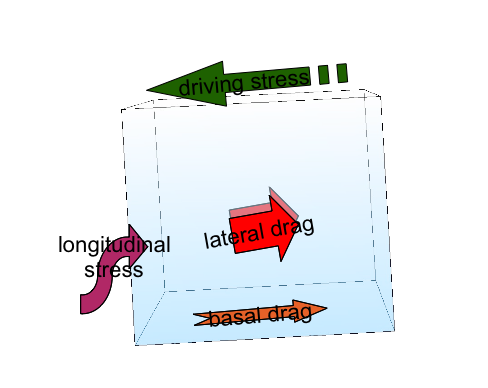
\includegraphics[width=0.5\columnwidth]{\dir/figs/StressBalance.eps}
  \end{center}
  \caption{The gravitational stress available to move the ice is the driving stress, indicated in green. Because the ice is assumed to be in equilibrium, the sum of the other stresses is equal to (i.e., must balance) the gravitational driving stress. In the 0-order model (shallow-ice approximation) the driving stress is assumed to be balanced by basal drag alone. In higher-order models, this restriction is relaxed and the balance of stresses now includes lateral and/or longitudinal stresses. Importantly, because these stresses must be computed based on conditions outside of the local computational cell (the local ice column), this significantly increases the complexity of the model.}
  \label{fig:stressbalance}
\end{figure} 

\begin{itemize}
\item For parts of the ice sheet that we are the most interested in -- e.g. ice streams, ice shelves, and other regions of fast flow -- horizontal-stress gradients are as or more important than vertical stress gradients. To model the flow in these regions accurately, higher-order models are required.

\item The shallow-ice approximation, applied to situations in which there is basal sliding, gives rise to a singularity in the the vertical velocity. Models compute the vertical velocity by integrating incompressibility.
\end{itemize}

\begin{align*}
\frac{\partial w}{\partial z} = -\frac{\partial u}{\partial x}-\frac{\partial v}{\partial y}
\end{align*}

\begin{description}
\item[]	If there is a jump from no-sliding in one grid cell to sliding in the one next to it, the horizontal velocity gradients at the bed will be entirely dependent on the grid spacing; the horizontal gradients (and through incompressibility, the vertical velocity gradient and thus the vertical velocity) will become increasingly large as the grid spacing decreases. Obviously, this is nonsensical and to be avoided.

\end{description}
\begin{itemize}
\item Incomplete knowledge of the stresses near the grounding line, which are often dominated by horizontal rather than vertical stresses, makes it unlikely that shallow ice models will ever be able to accurately simulate grounding line advance and retreat.

\item In some regions of very slow flow, like ice divides, horizontal-stress gradients are important or dominant. Ice cores are often recovered at ice divides and flow modeling is important for interpreting ice core records and using information (such as layer thickness) to infer the past flow history in the region. In order to model that flow correctly, one must include horizontal stresses (At an ice divide the surface slope is \(\sim\)0, in which case vertical stress gradients that drive deformation in 0-order models are also \(\sim\)0. In reality, deformation is not 0 at ice divides, it is simply controlled by horizontal stretching rather than vertical shearing).
\end{itemize}

The term higher-order comes from scaling analyses of the Stokes equations for which a scaling parameter $\lambda=H/L$ -- the ratio of the thickness to the horizontal length scale of interest -- is used to assign importance to the various terms. Shallow ice models retain only terms of order 0 while higher-order models also retain terms of order 1 (and possibly greater) (Figure \ref{fig:hoeqns}). 

\begin{figure}
  \begin{center}
    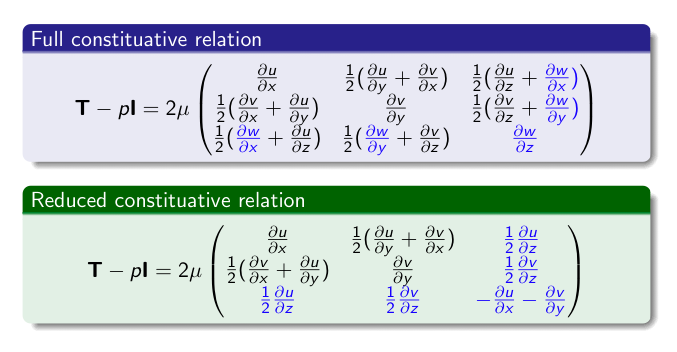
\includegraphics[width=0.7\columnwidth]{\dir/figs/HOeqns.eps}
   \end{center}
  \caption{Stokes-flow (top) and first-order (bottom) constitutive equations.}
  \label{fig:hoeqns}
\end{figure} 

\subsection{Available schemes}

\begin{itemize}
\item The most basic and fundamental higher-order scheme is the full, non-linear Stokes equations. Because of the computational burden, many 3d, large-scale models solve lower-order approximations to the Stokes equations (Figure \ref{fig:phylogeny}). However, a number of groups are making significant advances in this area and it seems likely that 3d, nonlinear-Stokes ice sheet models being used in climate-model applications is not far away (e.g. see the ELMER-Ice effort; \citet{gagliardini:2013iv}). Upcoming DOE-funded efforts will focus on implementing a nonlinear Stokes model on unstructured grids in CISM \citep{Leng:2012ia}.
\end{itemize}

\begin{itemize}
\item Probably the most long-lived higher-order approximation in glaciology is the shallow-shelf approxmation (or SSA) describing flow within an ice shelf (or ice stream if non-zero basal drag is included). It was made popular by Doug MacAyeal in the 80's and 90's (e.g., \citet{Macayeal:1989uo}). It's main disadvantage is that it is not fully 3d, as it assumes uniform velocity throughout the ice thickness driven only by horizontal stress gradients. It is, however, adequate for describing fast flow in many parts of the ice sheets, such as on ice shelves and along some ice streams. In this case, not resolving vertical gradients is a computational advantage.   
\end{itemize}

\begin{itemize}
\item The SSA equations are actually a depth-averaged form of a more general higher-order model, which is commonly referred to as the ``Blatter-Pattyn model" (\citet{BLATTER:1995wz}; \citet{Pattyn:2003tj}). This model has been around since the mid 90's and has become increasingly popular ever since. Blatter-Pattyn dynamics, synonymous with and more formally described as the ``first-order accurate Stokes approximation"\footnote{See \citet{Schoof:2010dl} and \citet{DUKOWICZ:2010wb} for a more complete scaling analysis and derivation of the first-order Stokes approximation.}, are currently implemented as the default higher-order dynamical core within CISM. 
\end{itemize}

\begin{itemize}
\item Several hybrid schemes exist that are computationally cheaper than the Blatter-Pattyn model. These combine solutions to the shallow ice approximation (for resolving vertical gradients) and the SSA approximation (for resolving horizontal gradients) in some clever way so that a fully 3d solution is obtained. It isn't yet known how well these model solutions compare to fully 3d models, or if one approach (hybrid vs. fully 3d solution) is superior to the other. David Pollard of Penn State and Ed Bueler of Univ. of Alaska Fairbanks currently run large-scale implementations of this type of model (\citet{Bueler:2009ee}; \citet{Pollard:2009ed}).
\end{itemize}

A good review paper that goes into a fair amount of detail about the various ice flow modeling approximations, their derivations, and their applicability, is the recent review by \citet{Schoof:2013is}.

\subsection{Practical differences between shallow ice models and higher-order models}

\begin{figure}
  \begin{center}
    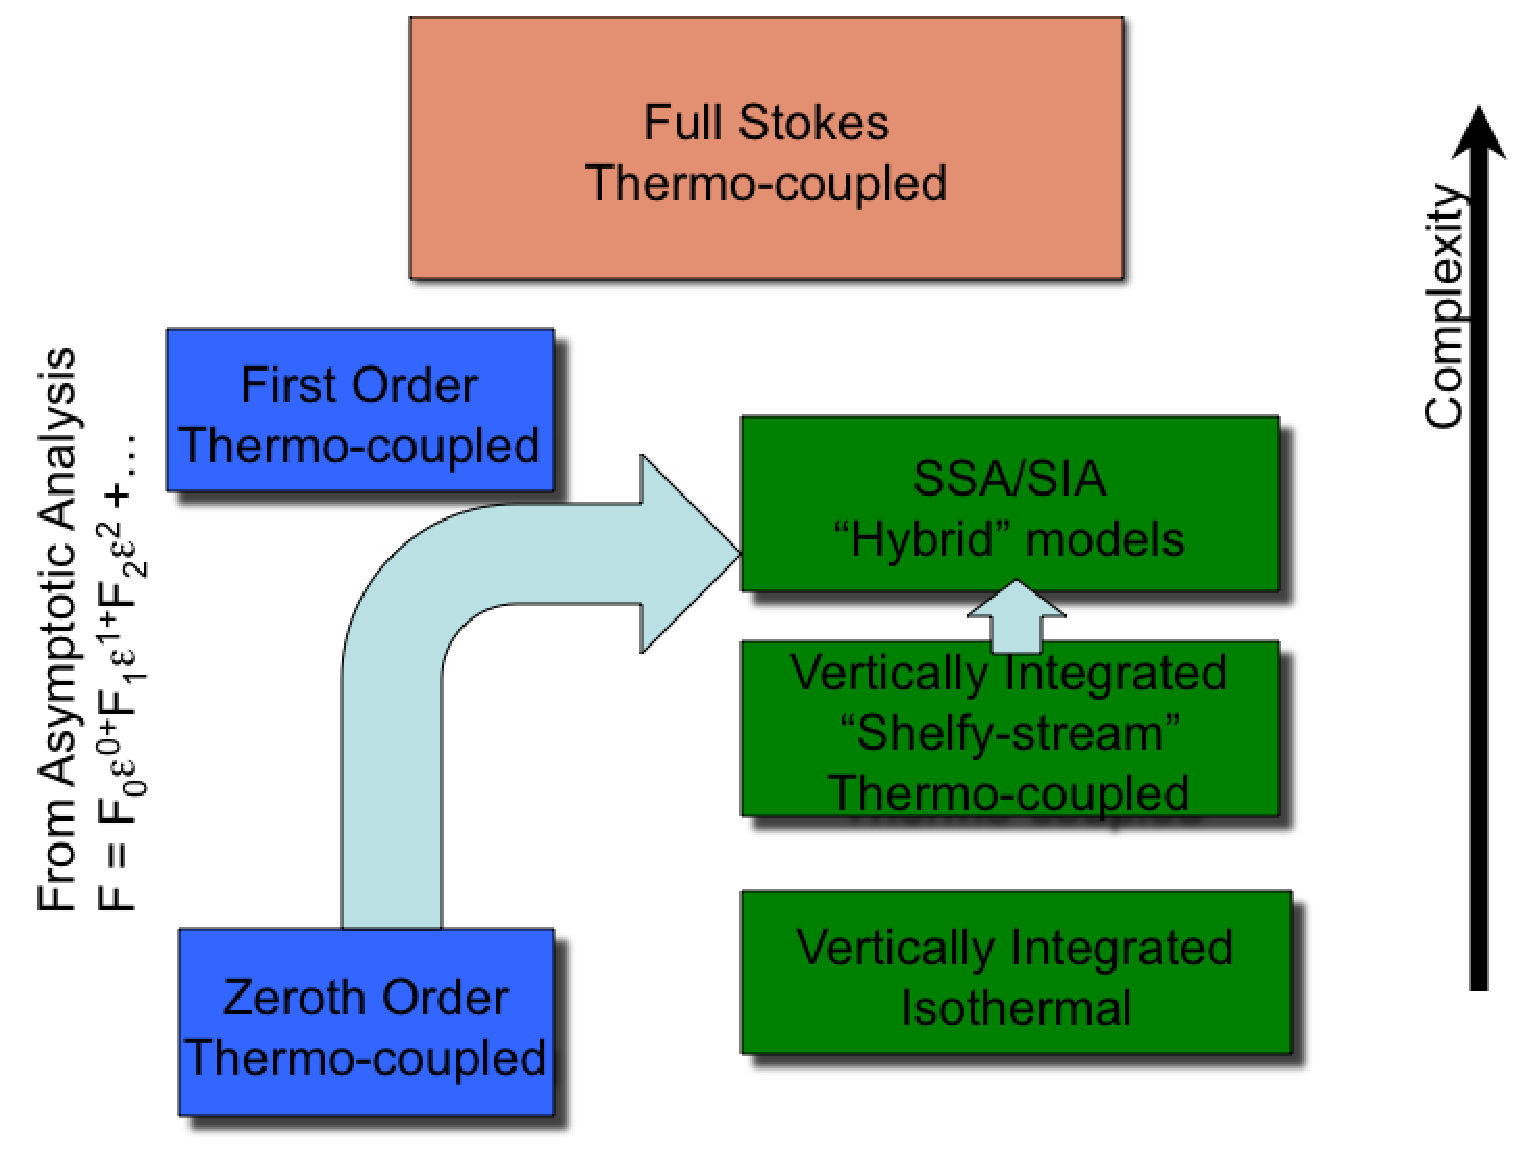
\includegraphics[width=0.5\columnwidth]{\dir/figs/ISMPhylogeny.eps}
   \end{center}
  \caption{The relationship between several common varieties of ice sheet modesl. Complexity increases along the vertical axis.}
   \label{fig:phylogeny}
\end{figure} 

By practical differences, we mean \textbf{(1)} how do we deal with solving the momentum equations in each case (the dynamics, or stress balance) and \textbf{(2)} how do we use the relevant information we derive from that solution (the kinematics, or velocity fields) to evolve the ice sheet geometry in time? There are large differences in how both of these issues are handled -- in shallow ice models versus in higher-order models -- for two main reasons:

\begin{itemize}
\item  The numerical solution of the dynamical equations is fundamentally different in each case. For the shallow ice case, we need only local information (slope and thickness) to solve for the velocity as a function of depth in a single column of ice. We do this pointwise for every location on our model domain (in map view), which is a relatively easy numerical problem; each column of velocities leads to a banded coefficient matrix that is relatively easy to invert (to solve for the velocities). This problem is also what we might call $embarrassingly$ $parallel$; in theory, each column of unknown velocities results in its own tridiagonal matrix, which could be solved for on its own processor. For higher-order models, however, we cannot do this since the solution at any point also depends on the solution at neighboring points (in map plane). The velocity at any point depends on non-local information, leading to an elliptic system of equations, and every velocity must be solved for simultaneously with every other velocity. The result is a much larger system of equations to solve, which is a more difficult numerical problem to solve on one processor and a much more difficult problem to solve on multiple processors. Because large-scale applications of higher-order models (e.g. whole-ice sheet models and coupling with climate models) will require efficient solution and parallelization techniques, this is a very active area of current research.  
\end{itemize}

\begin{itemize}
\item  The equations governing dynamics AND evolution in a shallow ice model can be recast together as a single, non-linear, diffusion equation for ice thickness. A single system of equations is solved to calculate the velocity field and evolve the ice sheet geometry. For higher-order models, we must first solve the momentum balance equations to obtain the velocity field. Then, we need to use some other scheme to evolve the ice thickness. 
\end{itemize}

Both of these differences mean that a model based on shallow ice physics may be built in a fundamentally different way than one based on higher-order physics. Most of the development work on CISM during the past few years has had to do with upgrading the model so that it can be used effectively and efficiently with higher-order dynamics schemes.  

The equations describing a (2d) higher-order flow that is vertically integrated (i.e., the SSA) are:

\begin{align*}
\frac{\partial}{\partial x}\left ( 2 \eta H 
\left(2\frac{\partial u}{\partial x}+\frac{\partial v}{\partial y}\right)\right)
+\frac{\partial}{\partial y}\left(\eta H\left(
\frac{\partial u}{\partial y}+\frac{\partial v}{\partial x}\right)\right)
=\rho_w gH \frac{\partial s}{\partial x}
\end{align*}


\begin{align*}
\frac{\partial}{\partial y}\left ( 2 \eta H 
\left(2\frac{\partial v}{\partial y}+\frac{\partial u}{\partial x}\right)\right)
+\frac{\partial}{\partial x}\left(\eta H\left(
\frac{\partial u}{\partial y}+\frac{\partial v}{\partial x}\right)\right)
=\rho_w gH \frac{\partial s}{\partial y}
\end{align*}

The equations describing a (3d) higher-order flow that is NOT vertically integrated (Blatter-Pattyn) are:

\begin{align*}
\frac{\partial}{\partial x}\left ( 2 \eta  
\left(2\frac{\partial u}{\partial x}+\frac{\partial v}{\partial y}\right)\right)
+\frac{\partial}{\partial y}\left(\eta \left(
\frac{\partial u}{\partial y}+\frac{\partial v}{\partial x}\right)\right)
+\frac{\partial}{\partial z}\left(\eta \frac{\partial u}{\partial z}\right)
=\rho_w g \frac{\partial s}{\partial x}
\end{align*}


\begin{align*}
\frac{\partial}{\partial y}\left ( 2 \eta 
\left(2\frac{\partial v}{\partial y}+\frac{\partial u}{\partial x}\right)\right)
+\frac{\partial}{\partial x}\left(\eta \left(
\frac{\partial u}{\partial y}+\frac{\partial v}{\partial x}\right)\right)
+\frac{\partial}{\partial z}\left(\eta \frac{\partial v}{\partial z}\right)
=\rho_w g \frac{\partial s}{\partial y}
\end{align*}

There are three differences that you should note
\begin{enumerate}
\item  The vertically integrated model includes the ice thickness, $H$, in each term. This is a reflection of the integration and does not appear in the first order equations.
\item  Accounting for the thickness not appearing, the only other difference is the presence of a vertical diffusion of horizontal velocities. This is the the third term on the left in the above equations.
\item  The first order equations must be solved on each of a set of horizontal layers. Layers communicate with each other through the vertical diffusion term.
\end{enumerate}

Both sets of equations are non-linear elliptical equations and much of the same technology can be used solve them. Additional complications come in when we account for boundary conditions at the lateral margins of the domain and at the upper and lower surfaces of the flow (note that for the vertically integrated flow, there are no explicit boundary conditions for the upper and lower surfaces; they are accounted for and incorporated during the vertical integration).

\subsection{Higher-order CISM}

\begin{figure}
  \begin{center}
    
\includegraphics[width=0.65\columnwidth]{\dir/figs/GIS.eps}
   \end{center}
  \caption{Observation-based balance velocities for Greenland (left) and depth-averaged speed from higher-order CISM (right) with basal sliding coefficients optimized to match the balance velocities (after Price et al., $PNAS$, \textbf{108}(22), 2011).}
  \label{fig:GIS_PNAS}
\end{figure} 

The higher-order dynamics scheme currently implemented in CISM (some output from which is shown in Figure \ref{fig:GIS_PNAS}) is discussed in more detail in the following chapters. First, the derivation of the equations themselves is discussed, followed by a discussion of the boundary conditions. Solutions methods for the nonlinear system of equations are then discussed. Finally, there is a brief discussion on the solution of the thickness evolution equation. 

A very useful higher-order model intercomparison project (ISMIP-HOM) was organized by Frank Pattyn from the Université Libre de Bruxelles. That project, which resulted in a set of "benchmark" experiments for higher-order models, is reported on formally in Pattyn et al. (2008). 

%\section{References}
%\begin{itemize}
%\item  \href{http://www.agu.org/journals/jf/jf0903/2008JF001179/}{Bueler, E. and J. Brown. Shallow shelf approximation as a "sliding law" in a thermomechanically coupled ice sheet model. \textit{J. Geophys. Res.}, F03008, doi:10.1029/2008JF001179, 2009.} 
%\item  \href{http://www.nature.com/nature/journal/v458/n7236/full/nature07809.html}{Pollard, D. and R.M. DeConto. Modelling West Antarctic ice sheet growth and collapse through the past five million years. \textit{Nature}, \textbf{458}, doi:10.1038/nature07809, 2009.}
%\item  \href{http://www.agu.org/journals/jb/jb0308/2002JB002329/}{Pattyn, F. A new three-dimensional higher-order thermomechanical ice sheet model: Basic sensitivity, ice stream development, and ice flow across subglacial lakes, \textit{J. Geophys. Res.}, \textbf{108}(B8), 2003.}
%\item  {Pattyn, F. and 20 others. Benchmark experiments for higher-order and full Stokes ice sheet models (ISMIP-HOM), \textit{The Cryosphere}, \textbf{2}, 2008.}
%\end{itemize}
%\end{document}

\section{Higher-Order Momentum Balance}
\label{sc:higher-order-mom}

\begin{figure}
  \begin{center}
    
\includegraphics[width=0.65\columnwidth]{\dir/figs/GIS.eps}
   \end{center}
  \caption{Observation-based balance velocities for Greenland (left) and depth-averaged speed from higher-order CISM (right) with basal sliding coefficients optimized to match the balance velocities (after Price et al., $PNAS$, \textbf{108}(22), 2011).}
  \label{fig:GIS_PNAS}
\end{figure} 

The higher-order dynamics scheme in CISM (some output from which is shown in Figure \ref{fig:GIS_PNAS}) is discussed in more detail in the following sections. 
First we describe the derivation of the equations themselves, followed by a discussion and derivation of the boundary conditions.
We then describe generic solution methods for the nonlinear system of equations, followed by a
brief discussion of the solution of the thickness evolution equation.

% Commented out the subsection because there are no other subsections in this section
%\subsection{Derivation of the Blatter-Pattyn Equations}
%\label{sc:higher-order-blatter-pattyn}

The higher-order dynamics scheme in CISM is based on the 3d first-order accurate Stokes approximation (also often referred to as the ``Blatter-Pattyn" model). The starting point is the nonlinear Stokes equations:

\begin{equation}
  \begin{split}
    & x:\quad \frac{\partial \tau _{xx}}{\partial x} + \frac{\partial \tau _{xy}}{\partial y} + \frac{\partial \tau _{xz}}{\partial z} - \frac{\partial P}{\partial x} = 0, \\ 
    & y:\quad \frac{\partial \tau _{xy}}{\partial x} + \frac{\partial \tau _{yy}}{\partial y} + \frac{\partial \tau _{yz}}{\partial z} - \frac{\partial P}{\partial y} = 0, \\ 
    & z:\quad \frac{\partial \tau _{xz}}{\partial x} + \frac{\partial \tau _{zy}}{\partial y} + \frac{\partial \tau _{zz}}{\partial z} - \frac{\partial P}{\partial z} = \rho_i g,
  \end{split}
\end{equation}

\noindent
where \textit{P} is the pressure and {\large \(\tau{}\)} is the deviatoric stress tensor. The latter is given by $\tau _{ij}=\sigma _{ij}+P\delta _{ij}$, 
where {\large \(\sigma{}\)} is the full stress tensor.

There are a number of ways to argue that, due to the shallowness of ice sheets (i.e., the small value of \textit{H}/\textit{L}, where \textit{H} is the thickness and \textit{L} is a relevant horizontal length scale), the Stokes equations can be reduced to the following first-order approximation:

\begin{equation}
  \begin{split}
    & x:\quad \frac{\partial \tau _{xx}}{\partial x} + \frac{\partial \tau _{xy}}{\partial y} + \frac{\partial \tau _{xz}}{\partial z} - \frac{\partial P}{\partial x} = 0, \\ 
    & y:\quad \frac{\partial \tau _{yy}}{\partial y} + \frac{\partial \tau _{xy}}{\partial x} + \frac{\partial \tau _{yz}}{\partial z} - \frac{\partial P}{\partial y} = 0, \\ 
    & z:\quad \frac{\partial \tau _{zz}}{\partial z} - \frac{\partial P}{\partial z} = \rho g. \\ 
  \end{split}
\end{equation}

\noindent
The arguments supporting this reduction are fairly complex and are based on either a variational analysis or an asymptotic analysis (see \citet{Schoof:2010dl} and \citet{DUKOWICZ:2010wb} for details).

The third (vertical) balance equation above can be integrated vertically to give an expression for the pressure:
\begin{equation}
P = \rho g\left( s-z \right) + \tau _{zz}(z).
\end{equation} 
This is simply a statement that the full vertical normal stress is balanced by the hydrostatic pressure (the so-called \textit{hydrostatic assumption}). This expression can be substituted into the horizontal pressure gradient terms above to remove pressure from the equations. For example, for the \textit{x} component of velocity we have

\begin{equation}
  \label{ho.eq.x_stress_balance}
  \begin{split}
    & \frac{\partial \tau _{xx}}{\partial x} + \frac{\partial \tau _{xy}}{\partial y} + \frac{\partial \tau _{xz}}{\partial z} = \frac{\partial }{\partial x}\left[ \rho g\left( s-z \right)+\tau _{zz}(z) \right] \\ 
    & \frac{\partial \tau _{xx}}{\partial x} - \frac{\partial \tau _{zz}}{\partial x} + \frac{\partial \tau _{xy}}{\partial y} + \frac{\partial \tau _{xz}}{\partial z} = \rho g\frac{\partial s}{\partial x} \\ 
  \end{split}
\end{equation}

\noindent
Using the incompressibility constraint \eqref{ho.eq.incompress} and the assumption that stress and strain are aligned we can write

\begin{equation}
  \label{ho.eq.incompress_tau}
  \tau _{zz} = -\tau _{xx}-\tau _{yy}.
\end{equation}

\noindent
Taking the gradient of \eqref{ho.eq.incompress_tau} with respect to $x$, we can rewrite the vertical normal deviatoric stress in terms of horizontal normal deviatoric stresses:

\begin{equation}
  \label{ho.eq.incompress_tau_dx}
  -\frac{\partial \tau _{zz}}{\partial x} = -\frac{\partial }{\partial x}\left( -\tau _{xx} - \tau _{yy} \right) = \frac{\partial \tau _{xx}}{\partial x} + \frac{\partial \tau _{yy}}{\partial x}.
\end{equation}
 
\noindent
Substituting \eqref{ho.eq.incompress_tau_dx} into \eqref{ho.eq.x_stress_balance}, we obtain
 
\begin{equation}
%  2\frac{\partial \tau _{xx}}{\partial x} + \frac{\partial \tau _{yy}}{\partial x} + \frac{\partial \tau _{xy}}{\partial y} + \frac{\partial \tau _{xz}}{\partial z} = \rho g\frac{\partial s}{\partial x}.
  \label{ho.eq.stress_balance_x}
  \frac{\partial }{\partial x} \left( 2 \tau_{xx} + \tau_{yy} \right) + \frac{\partial \tau _{xy}}{\partial y} + \frac{\partial \tau _{xz}}{\partial z} = \rho g\frac{\partial s}{\partial x}.
\end{equation}

\noindent
Similarly, the $y$ horizontal balance equation is
\begin{equation}
  \label{ho.eq.stress_balance_y}
  \frac{\partial }{\partial y} \left( 2 \tau_{yy} + \tau_{xx} \right) + \frac{\partial \tau _{xy}}{\partial x} + \frac{\partial \tau _{yz}}{\partial z} = \rho g\frac{\partial s}{\partial y}.
\end{equation}

\noindent 
At this point we have removed the vertical balance equation entirely; it has been incorporated into the horizontal balance equations through incompressibility.


%\begin{align*}
%  & x:\quad 2\frac{\partial \tau _{xx}}{\partial x}+\frac{\partial \tau _{yy}}{\partial x}+\frac{\partial \tau _{xy}}{\partial y}+\frac{\partial \tau _{xz}}{\partial z}=\rho g\frac{\partial s}{\partial x}\quad,  \\ 
% & y:\quad 2\frac{\partial \tau _{yy}}{\partial y}+\frac{\partial \tau _{xx}}{\partial y}+\frac{\partial \tau _{xy}}{\partial x}+\frac{\partial \tau _{yz}}{\partial z}=\rho g\frac{\partial s}{\partial y}. \\
%\end{align*}

Next we want to write these equations in terms of the velocities for which we are ultimately solving. Stresses and velocities are linked through the 
constitutive law for ice, which relates strain rates to stresses (here we assume Nye's generalization of Glen's law), and through the 
definition of the strain rate tensor, which relates strain rates to velocity gradients:

\begin{equation}
  \begin{split}
    & 1.\quad \tau _{ij}=B\dot{\varepsilon }_{e}^{\frac{1-n}{n}}\dot{\varepsilon }_{ij},\quad B=B(T) \\ 
    & 2.\quad \dot{\varepsilon }_{ij}=\frac{1}{2}\left( \frac{\partial u_{i}}{\partial x_{j}}+\frac{\partial u_{j}}{\partial x_{i}} \right) \\ 
    & 3.\quad 2\dot{\varepsilon }_{e}=\dot{\varepsilon }_{ij}\dot{\varepsilon }_{ij} \\ 
    & 4.\quad \eta \equiv \frac{1}{2}B\dot{\varepsilon }_{e}^{\frac{1-n}{n}} \\ 
    & 5.\quad \tau _{ij}=2\eta \dot{\varepsilon }_{ij} \\ 
  \end{split}
\end{equation}

\noindent
In order, the five expressions above give: 

\begin{enumerate}
\item  Glen's flow law\footnote{Technically, we are using the \textit{inverse} form of the flow-law here.}, where 
$B = A^{\frac{-1}{n}}$ is the temperature dependent rate factor 
\item  The definition of the strain-rate tensor in terms of velocity gradients
\item  The definition of the effective strain rate, $\dot{\varepsilon }_{e}$, a norm of the strain-rate tensor
\item  A definition of the ``effective viscosity" (after rearranging some terms in (1))
\item  Items (1)-(4) allow us to write the relationship between stress and strain in a standard ``Newtonian" way, but with a non-Newtonian (nonlinear) viscosity
\end{enumerate}

\noindent
Now, taking these definitions into the stress balance equations \eqref{ho.eq.stress_balance_x} and \eqref{ho.eq.stress_balance_y} 
and expanding in terms of strain rates and effective viscosity, we have (for the \textit{x} direction only):

\begin{equation}
  x: \quad 2\frac{\partial }{\partial x}\left( 2\eta \dot{\varepsilon }_{xx} \right) + \frac{\partial }{\partial x}\left( 2\eta \dot{\varepsilon }_{yy
} \right) + \frac{\partial }{\partial y}\left( 2\eta \dot{\varepsilon }_{xy} \right) + \frac{\partial }{\partial z}\left( 2\eta \dot{\varepsilon }_{xz} 
\right) = \rho g\frac{\partial s}{\partial x}, \\ 
%  x: \quad 2\frac{\partial }{\partial x} \left( 2\eta \dot{\varepsilon }_{xx} +  2\eta \dot{\varepsilon}_{yy} \right) +\frac{\partial }{\partial y}\left( 2\eta \dot{\varepsilon }_{xy} \right)+\frac{\partial }{\partial z}\left( 2\eta \dot{\varepsilon }_{xz} \right)=\rho g\frac{\partial s}{\partial x}. \\ 
\end{equation}

\noindent
Replacing strain-rate components with velocity gradients, we obtain

\begin{equation}
  \label{ho.eq.stress_balance_final_x}
  x: \quad \frac{\partial }{\partial x}\left( 4 \eta \frac{\partial u}{\partial x} +  2 \eta \frac{\partial v}{\partial y} \right) + \frac{\partial }{\partial y}\left[ \eta \left( \frac{\partial u}{\partial y} + \frac{\partial v}{\partial x} \right) \right]+\frac{\partial }{\partial z}\left( \eta \frac{\partial u}{\partial z} \right) = \rho g\frac{\partial s}{\partial x}.
\end{equation}

\noindent
An analogous expression gives the \textit{y}-direction momentum balance: 

\begin{equation}
  \label{ho.eq.stress_balance_final_y}
  y: \quad \frac{\partial }{\partial y}\left( 4 \eta \frac{\partial v}{\partial y} +  2 \eta \frac{\partial u}{\partial x} \right) + \frac{\partial }{\partial x}\left[ \eta \left( \frac{\partial u}{\partial y} + \frac{\partial v}{\partial x} \right) \right]+\frac{\partial }{\partial z}\left( \eta \frac{\partial v}{\partial z} \right) = \rho g\frac{\partial s}{\partial y}.  
\end{equation}

\noindent
These are the basic equations to be discretized and solved.

%Thus, the final form of the equations to be discretized and solved is given by:

%\begin{align*}
%  & x:\quad 4\frac{\partial }{\partial x}\left( \eta \frac{\partial u}{\partial x} \right)+\frac{\partial }{\partial y}\left( \eta \frac{\partial u}{\partial y} \right)
%  +2\frac{\partial }{\partial x}\left( \eta \frac{\partial v}{\partial y} \right)+\frac{\partial }{\partial y}\left( \eta \frac{\partial v}{\partial x} \right)
%  +\frac{\partial }{\partial z}\left( \eta \frac{\partial u}{\partial z} \right)=\rho g\frac{\partial s}{\partial x}, \\ 
% & y:\quad 4\frac{\partial }{\partial y}\left( \eta \frac{\partial v}{\partial y} \right)+\frac{\partial }{\partial x}\left( \eta \frac{\partial v}{\partial x} \right)
% +2\frac{\partial }{\partial y}\left( \eta \frac{\partial u}{\partial x} \right)+\frac{\partial }{\partial x}\left( \eta \frac{\partial u}{\partial y} \right)
% +\frac{\partial }{\partial z}\left( \eta \frac{\partial v}{\partial z} \right)=\rho g\frac{\partial s}{\partial y}. \\ 
%\end{align*}


\section{Higher-Order Model Boundary Conditions}
\label{sc:higher-order-bcs}

We now carry out an approximate derivation of the boundary conditions that are implemented with CISM's higher-order scheme. By approximate we mean that some of the derivation is guided by physical intuition and reasonable arguments, rather than rigorous mathematics. In the end, we derive the same set of equations as when following the more rigorous approach (see, e.g. \citet{DUKOWICZ:2010wb}). We will look at the derivation in three parts, (1) the free surface boundary condition, (2) the basal traction boundary condition, and (3) lateral boundary conditions.

\subsection{Stress-free Surface}
At the upper ice surface, a stress-free boundary condition is applied. The traction vector $T_i$ must be continuous across the ice sheet surface and, assuming that atmospheric pressure and surface tension are small, we have

\begin{equation}
  \label{ho.eq.surface_traction}
  \begin{split}
    & T_{i} = -T_{i(\textrm{boundary})}\approx 0, \\ 
    & T_{i} = \sigma _{ij}n_{j} = \sigma _{i1}n_{1} + \sigma _{i2}n_{2} + \sigma _{i3}n_{3} = 0, \\
  \end{split}
\end{equation}

\noindent
where the $n_i$ are the components of the outward facing, unit normal vector in Cartesian coordinates.

For a function \textit{F(x,y,z) = z -- f(x,y) = 0}, where \textit{z = f(x,y)} defines the surface, the gradient of \textit{F(x,y,z)} gives the components of the surface normal vector. For the case of the ice sheet surface, $s = f(x,y)$ and the surface normal is given by

\begin{equation}
  n_{i}=\left( -\frac{\partial s}{\partial x},-\frac{\partial s}{\partial y},1 \right)\frac{1}{a},
\end{equation}

\noindent
where

\begin{equation}
  a = \sqrt{\left( \frac{\partial s}{\partial x} \right)^{2} + \left( \frac{\partial s}{\partial y} \right)^{2} + 1}.
\end{equation}

\noindent
Eq. \eqref{ho.eq.surface_traction} gives three equations that must be satisfied at the free surface:

\begin{equation}
  \begin{split}
    & i=x: \quad T_{x} = \sigma _{xx}n_{x} + \sigma _{xy}n_{y} + \sigma _{xz}n_{z}=0, \\ 
    & i=y: \quad T_{y} = \sigma _{yx}n_{x} + \sigma _{yy}n_{y} + \sigma _{yz}n_{z}=0, \\ 
    & i=z: \quad T_{z} = \sigma _{zx}n_{x} + \sigma _{zy}n_{y} + \sigma _{zz}n_{z}=0. \\ 
  \end{split}
\end{equation}

\noindent
Expanding the $z$ equation and expressing stresses in terms of strain rates and pressures, where $\eta$ is the effective viscosity defined above, gives

\begin{equation}
  \left( 2\eta \dot{\varepsilon }_{zx} \right)n_{x}+\left( 2\eta \dot{\varepsilon }_{zy} \right)n_{y}+\left( 2\eta \dot{\varepsilon }_{zz}-P \right)n_{z}=0.
\end{equation}

\noindent
Solving for the pressure gives

\begin{equation}
  Pn_{z} = \left( 2\eta \dot{\varepsilon }_{zz} \right)n_{z}+\left( 2\eta \dot{\varepsilon }_{zx} \right)n_{x}+\left( 2\eta \dot{\varepsilon }_{zy} \right)n_{y}.
\end{equation}

\noindent
Expanding in terms of velocity gradients and normal vector components, we find

\begin{equation}
  P = 2\eta \frac{\partial w}{\partial z}-\left( \eta \frac{\partial u}{\partial z} \right)\frac{\partial s}{\partial x}-\left( \eta \frac{\partial v}{\partial z} \right)\frac{\partial s}{\partial y},
\end{equation}

where we have made the usual first-order approximation that 

\begin{equation}
  \frac{\partial w}{\partial x}=\frac{\partial w}{\partial y}\approx 0.
\end{equation}

\noindent
\textit{(WHL: and also assumed $a \approx 1$?)}

\textbf{WHL: The rest of this section derives BC discretizations that were used in Glam but are not necessary
in a finite-element approach. So I think the remaining text could be rewritten a bit and considerably shortened.}

We use this expression for the pressure and expand the two horizontal boundary condition expressions

\begin{equation}
\begin{split}
 & i=x:\quad T_{x}=\sigma _{xx}n_{x}+\sigma _{xy}n_{y}+\sigma _{xz}n_{z}=0, \\ 
 & i=y:\quad T_{y}=\sigma _{yx}n_{x}+\sigma _{yy}n_{y}+\sigma _{yz}n_{z}=0, \\
\end{split}
 \end{equation}

in terms of velocity gradients and the effective viscosity to obtain

\begin{equation}
\begin{split}
   {} & \hat{x}:\quad -2\eta \frac{\partial u}{\partial x}\frac{\partial s}{\partial x}-\eta \left( \frac{\partial u}{\partial y}+\frac{\partial v}{\partial x} \right)\frac{\partial s}{\partial y}+\eta \frac{\partial u}{\partial z}=  \\
   {} & \quad \quad \quad \quad \quad -2\eta \frac{\partial w}{\partial z}\frac{\partial s}{\partial x}+\eta \frac{\partial u}{\partial z}\left[ \frac{\partial s}{\partial x}\frac{\partial s}{\partial x} \right]+\eta \frac{\partial v}{\partial z}\left[ \frac{\partial s}{\partial y}\frac{\partial s}{\partial x} \right],  \\
%\end{equation}
%
%\begin{equation}
   {} & \hat{y}:\quad -2\eta \frac{\partial v}{\partial y}\frac{\partial s}{\partial y}-\eta \left( \frac{\partial u}{\partial y}+\frac{\partial v}{\partial x} \right)\frac{\partial s}{\partial x}+\eta \frac{\partial v}{\partial z}=  \\
   {} & \quad \quad \quad \quad \quad -2\eta \frac{\partial w}{\partial z}\frac{\partial s}{\partial y}+\eta \frac{\partial u}{\partial z}\left[ \frac{\partial s}{\partial x}\frac{\partial s}{\partial y} \right]+\eta \frac{\partial v}{\partial z}\left[ \frac{\partial s}{\partial y}\frac{\partial s}{\partial y} \right].  \\
\end{split}
\end{equation}

In both of these expression, the terms in square brackets are $\sim{0}$ (because slopes on ice sheets are small and the slope squared is exceedingly small). From continuity, we also have

\begin{equation}
\frac{\partial w}{\partial z}=-\frac{\partial u}{\partial x}-\frac{\partial v}{\partial y}.
\end{equation}

Using this expression for the normal vertical velocity gradient and removing the terms in square brackets our two horizontal boundary condition expressions become

\begin{equation}
\begin{split}
   {} & \hat{x}:\quad -2\eta \frac{\partial u}{\partial x}\frac{\partial s}{\partial x}-\eta \left( \frac{\partial u}{\partial y}+\frac{\partial v}{\partial x} \right)\frac{\partial s}{\partial y}+\eta \frac{\partial u}{\partial z}=2\eta \left( \frac{\partial u}{\partial x}\frac{\partial s}{\partial x}+\frac{\partial v}{\partial y}\frac{\partial s}{\partial x} \right),  \\
   {} & \hat{y}:\quad -2\eta \frac{\partial v}{\partial y}\frac{\partial s}{\partial y}-\eta \left( \frac{\partial u}{\partial y}+\frac{\partial v}{\partial x} \right)\frac{\partial s}{\partial x}+\eta \frac{\partial v}{\partial z}=2\eta \left( \frac{\partial u}{\partial x}\frac{\partial s}{\partial y}+\frac{\partial v}{\partial y}\frac{\partial s}{\partial y} \right).  \\
\end{split}
\end{equation}

%As in the derivation of the 1st-order stress balance equations, collect terms of a particular velocity gradient (that is, \textit{u} or \textit{v}) and move them to one side of the equation 
Moving terms to one side and dividing through by the effective viscosity \textit{\(\eta{}\)}, we arrive at the final form of the 1st-order, free surface boundary conditions

\begin{equation}
\begin{split}
   {} & \hat{x}:\quad 4\frac{\partial u}{\partial x}\frac{\partial s}{\partial x}+\frac{\partial u}{\partial y}\frac{\partial s}{\partial y}+2\frac{\partial v}{\partial y}\frac{\partial s}{\partial x}+\frac{\partial v}{\partial x}\frac{\partial s}{\partial y}-\frac{\partial u}{\partial z}=0,  \\
   {} & \hat{y}:\quad 4\frac{\partial v}{\partial y}\frac{\partial s}{\partial y}+\frac{\partial v}{\partial x}\frac{\partial s}{\partial x}+2\frac{\partial u}{\partial x}\frac{\partial s}{\partial y}+\frac{\partial u}{\partial y}\frac{\partial s}{\partial x}-\frac{\partial v}{\partial z}=0.  \\
\end{split}
\end{equation}

\subsection{Specified Basal Traction}
Derivation of the basal boundary condition follows that above for the free surface except that,
\begin{enumerate}

\item the right-hand side of the equation is not zero, rather it consists of an assumed basal traction vector with components 
\begin{equation}
\tau_{bi} = \left( \tau _{bx},\tau _{by} \right),
\end{equation}

\item the outward facing normal vector components now consist of horizontal gradients in the basal surface (with a resulting sign switch on the $x,y,z$ components relative to the upper surface)

\item the effective viscosity does not disappear from the equations when we divide through
\end{enumerate}

Making these substitutions we obtain the 1st-order basal boundary conditions for a specified basal traction

\begin{equation}
\begin{split}
  & \hat{x}:\quad 4\frac{\partial u}{\partial x}\frac{\partial b}{\partial x}+\frac{\partial u}{\partial y}\frac{\partial b}{\partial y}+2\frac{\partial v}{\partial y}\frac{\partial b}{\partial x}+\frac{\partial v}{\partial x}\frac{\partial b}{\partial y}-\frac{\partial u}{\partial z}=\frac{\tau _{bx}}{\eta }, \\ 
 & \hat{y}:\quad 4\frac{\partial v}{\partial y}\frac{\partial b}{\partial y}+\frac{\partial v}{\partial x}\frac{\partial b}{\partial x}+2\frac{\partial u}{\partial x}\frac{\partial b}{\partial y}+\frac{\partial u}{\partial y}\frac{\partial b}{\partial x}-\frac{\partial v}{\partial z}=\frac{\tau _{by}}{\eta }. \\
\end{split}
 \end{equation}

We assume that basal traction is linearly related to basal sliding velocity through a positive traction parameter, $\beta$, such that

\begin{equation}
\label{basaltraction}
\tau _{bx}=\left. -\beta u \right|_{z=b},\quad \tau _{by}=\left. -\beta v \right|_{z=b}.
\end{equation}

Note that the negative sign in front of the $\beta$ indicates that the traction vector is oriented parallel to and in the opposite direction of the sliding velocity vector.

Substituting this expression into the above gives our final horizontal boundary conditions at the ice sheet base

\begin{equation}
\begin{split}
  & \hat{x}:\quad 4\frac{\partial u}{\partial x}\frac{\partial b}{\partial x}+\frac{\partial u}{\partial y}\frac{\partial b}{\partial y}+2\frac{\partial v}{\partial y}\frac{\partial b}{\partial x}+\frac{\partial v}{\partial x}\frac{\partial b}{\partial y}-\frac{\partial u}{\partial z}+\left( \frac{B}{\eta } \right)u=0, \\ 
 & \hat{y}:\quad 4\frac{\partial v}{\partial y}\frac{\partial b}{\partial y}+\frac{\partial v}{\partial x}\frac{\partial b}{\partial x}+2\frac{\partial u}{\partial x}\frac{\partial b}{\partial y}+\frac{\partial u}{\partial y}\frac{\partial b}{\partial x}-\frac{\partial v}{\partial z}+\left( \frac{B}{\eta } \right)v=0. \\
\end{split}
 \end{equation}

The use of a linear traction parameter (Eq. \ref{basaltraction}) can be modified to
implement basal friction laws that are a function of effective pressure 
(ice overburden pressure minus water pressure at the bed) and 
(generally) nonlinear in the sliding velocity.  Two such basal friction laws are
implemented in CISM.  For friction laws that are nonlinear in sliding velocity,
$\beta$ in eq. \ref{basaltraction} becomes a function of sliding velocity.  This is
implemented by lagging the value of sliding velocity used to calculate an ``effective'' 
$\beta$ in the fixed-point iterations used to solve the momentum balance.

The first is a Weertman-style friction law \citep{Weertman1957, Weertman1964} modified 
to include an effective pressure dependence \citep{Bindschadler1983, Budd1979}.
Notation here follows the summary by \citet[][p.240, eq.7.17]{Cuffey2010}.  The form of
the friction law is:
\begin{equation}
  \label{weertmansliding}
  \vec{u_b} = k \vec{\tau_{b}}^p N^{-q}
\end{equation}
which can be rearranged for $\vec{\tau_b}$ as:
\begin{equation}
  \label{weertmansliding2}
  \vec{\tau_b} = k^\frac{-1}{p} \vec{u_b}^\frac{1}{p} N^\frac{q}{p}
\end{equation}
where $k$ is a friction coefficient based on thermal and mechanical properties of ice 
and inversely related to bed roughness.  \citet{Cuffey2010} suggest values of 
$p=3$ and $q=1$, making this nonlinear in velocity.  

One problem with Eq. \ref{weertmansliding} is that it allows for unbounded basal traction.
An improvement to this is a physically-based basal friction law for sliding over 
hard beds that allows for cavitation and bounded basal drag \citep[]{Schoof2005}, 
the second friction law in CISM that accounts for effective pressure: 
\begin{equation}
    \label{CF-law}
	  \vec{\tau_b} = C \left( \frac{ \vec{u_b} } { \vec{u_b} + N^n \Lambda} \right)^{1/n} N,   \Lambda=\frac{\lambda_{max}A}{m_{max}}
\end{equation}
In Eq. \ref{CF-law}, $C$ is a Coulomb friction coefficient,  and $\lambda_{max}$ and 
$m_{max}$ are the wavelength (m) and maximum slope, respectively, of the 
dominant bedrock bumps.  Near cavitation (i.e., when effective pressure approaches 
0 at high water pressure), the friction law becomes a Coulomb friction law of the 
form $\vec{\tau_b}=CN$. Alternatively, at large effective pressures (low water pressure) 
the friction law takes a power law form, $\vec{\tau_b} \propto u_b^{1/n}$. 
The representation of bump geometry in the friction law is at a sub-grid scale 
and not explicitly resolved in the grid geometry used by the model.

[Note that the release version of CISM does not currently include a hydrology model
that outputs effective pressure, so at present effective pressure fields must be
input as data to use these two basal friction laws.]

\subsection{Specified Basal Yield Stress}
The above implementation of a specified basal traction can be altered to simulate sliding over a sediment-covered bed for which the sediment has a plastic or ``Coulomb friction" rheology. That is, sliding does not occur below the specified yield stress of the underlying material (e.g., a water saturated subglacial till). When the yield stress, $\tau_0$ is reached, sliding occurs at a rate that maintains but does not exceed that yield stress. Consider the \textit{x} direction boundary condition above, written out in terms of basal stress components,

\begin{equation}
\begin{split}
  & \hat{x}:\quad 4\eta \frac{\partial u}{\partial x}\frac{\partial b}{\partial x}+\eta \frac{\partial u}{\partial y}\frac{\partial b}{\partial y}+2\eta \frac{\partial v}{\partial y}\frac{\partial b}{\partial x}+\eta \frac{\partial v}{\partial x}\frac{\partial b}{\partial y}-\eta \frac{\partial u}{\partial z}=\tau _{bx}, \\ 
 & \quad \quad \quad \quad \quad \quad \tau _{bx}\approx \tau _{0}=\tau _{0}\left( \frac{u}{\left| \mathbf{u} \right|} \right)=\tau _{0}\left( \frac{u}{\sqrt{u_{0}^{2}+v_{0}^{2}+\gamma }} \right) \\ 
\end{split}
\end{equation}

In the expression above, $u$ is the $x$ component of the basal sliding velocity from the current iteration, $u_0$ and $v_0$ are components from the previous iteration, and $\gamma$ is a regularization constant (a small constant number to avoid division by zero during early iterations). Note that as the solution converges, velocities at the current and previous iteration are nearly equal, and the expression in parentheses approaches 1, in which case the basal stress and yield stress are approximately equal. 

We can accommodate this into our earlier framework for incorporating the traction parameter $\beta$ by treating $\beta$ as being nonlinear and dependent on the velocity,

\begin{equation}
\begin{split}
  & \tau _{bx}=-\beta u,\quad \quad  \\ 
 & \beta \equiv \frac{\tau _{0}}{\sqrt{u_{0}^{2}+v_{0}^{2}+\gamma }},\quad  \\ 
 & \tau _{bx}=-\left( \frac{\tau _{0}}{\sqrt{u_{0}^{2}+v_{0}^{2}+\gamma }} \right)u.\quad  \\
\end{split}
\end{equation}

Thus, we can implement plastic bed sliding behavior simply by substituting the above expression for our ``nonlinear" \textit{{\large \(\beta{}\)}} into our previous expressions for the basal boundary conditions in \textit{x} (a similar expression applies for the \textit{y} direction). 
%Figures \ref{fig:plasticbed1} and \ref{fig:plasticbed2} below show some examples of this type of boundary condition for the case of an idealized ice stream.
Figure \ref{fig:plasticbed1} shows an example of this type of boundary condition for the case of an idealized ice stream simulated by CISM.

\begin{figure}
  \begin{center}
    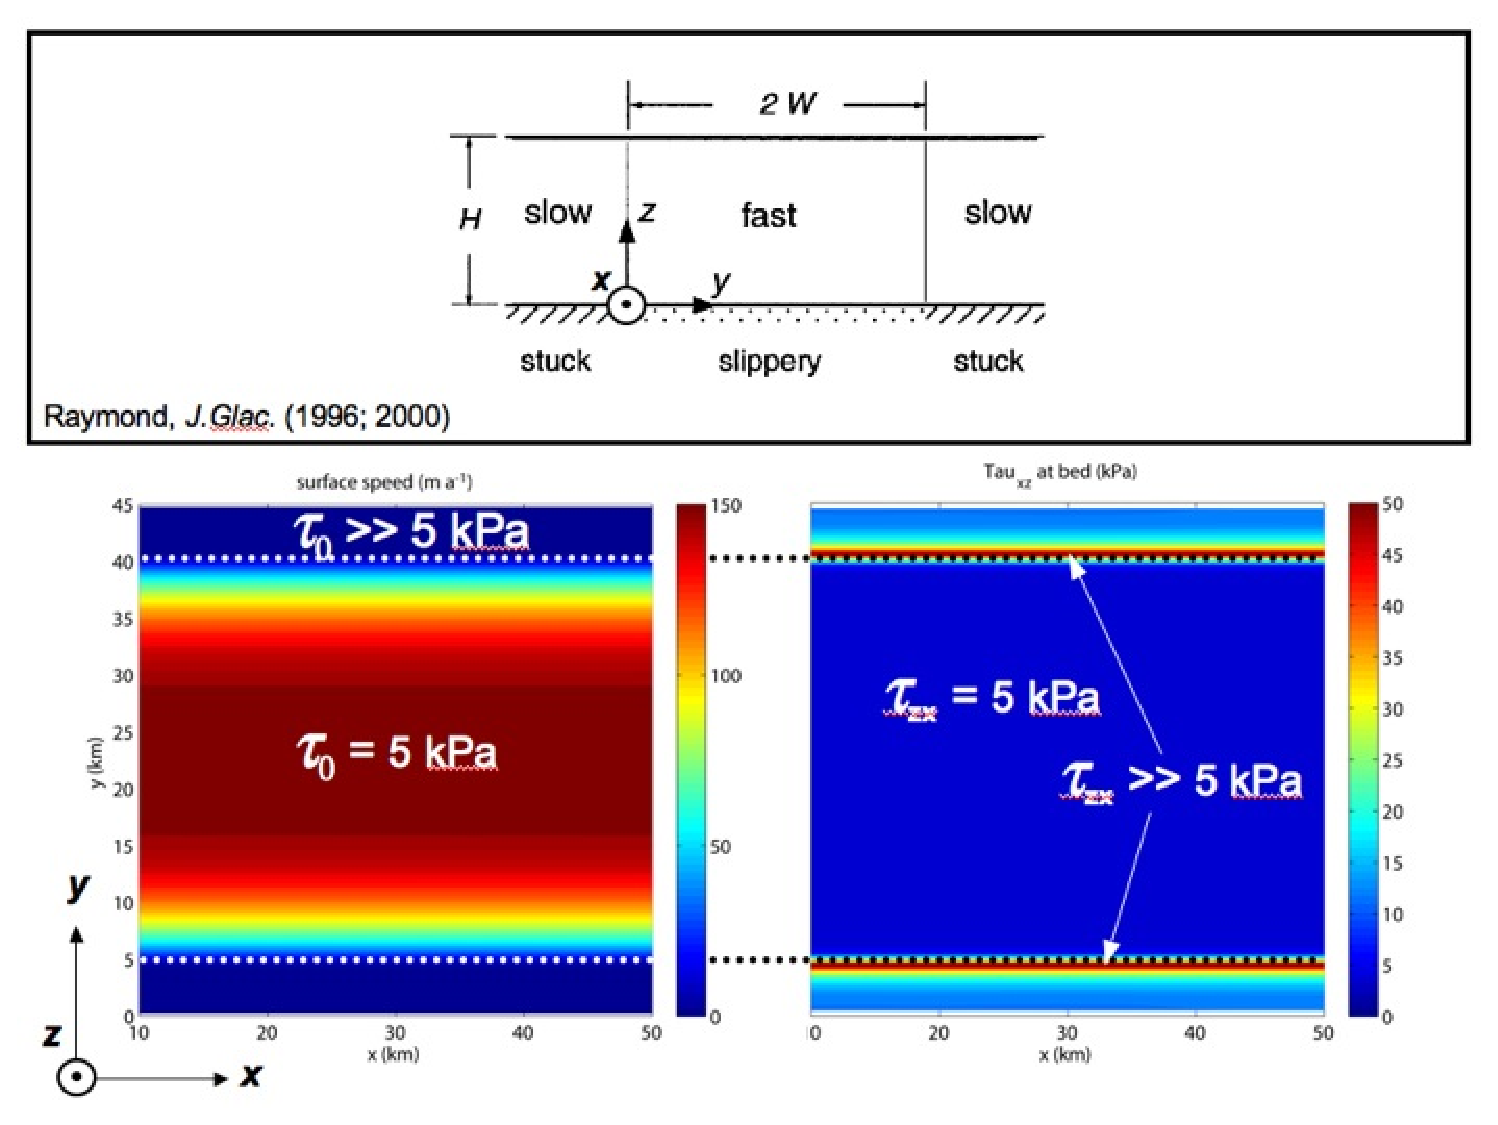
\includegraphics[width=0.65\columnwidth]{\dir/figs/Plastic_bed1.eps}
  \end{center}
  \caption{Idealized ice stream with plastic-bed sliding. Top panel shows a schematic of an idealized ice stream, frozen at the margins and thawed within the ice stream (flow is out of the page). Bottom panel (color) shows a modeled, idealized ice stream (flow is from left to right) with a yield stress of 5 kPa within the ice stream and much larger than 5 kPa outside of it. Bottom left shows the ice stream speed (m/yr) and the bottom right shows the basal drag (kPa). Within the ice stream basal drag is equal to the yield stress. Outside of the ice stream, stress transfer to the lateral margins results in basal drag that is much larger than the yield stress (and also much larger than the driving stress).}
  \label{fig:plasticbed1}
\end{figure} 

%\begin{figure}
%  \begin{center}
%    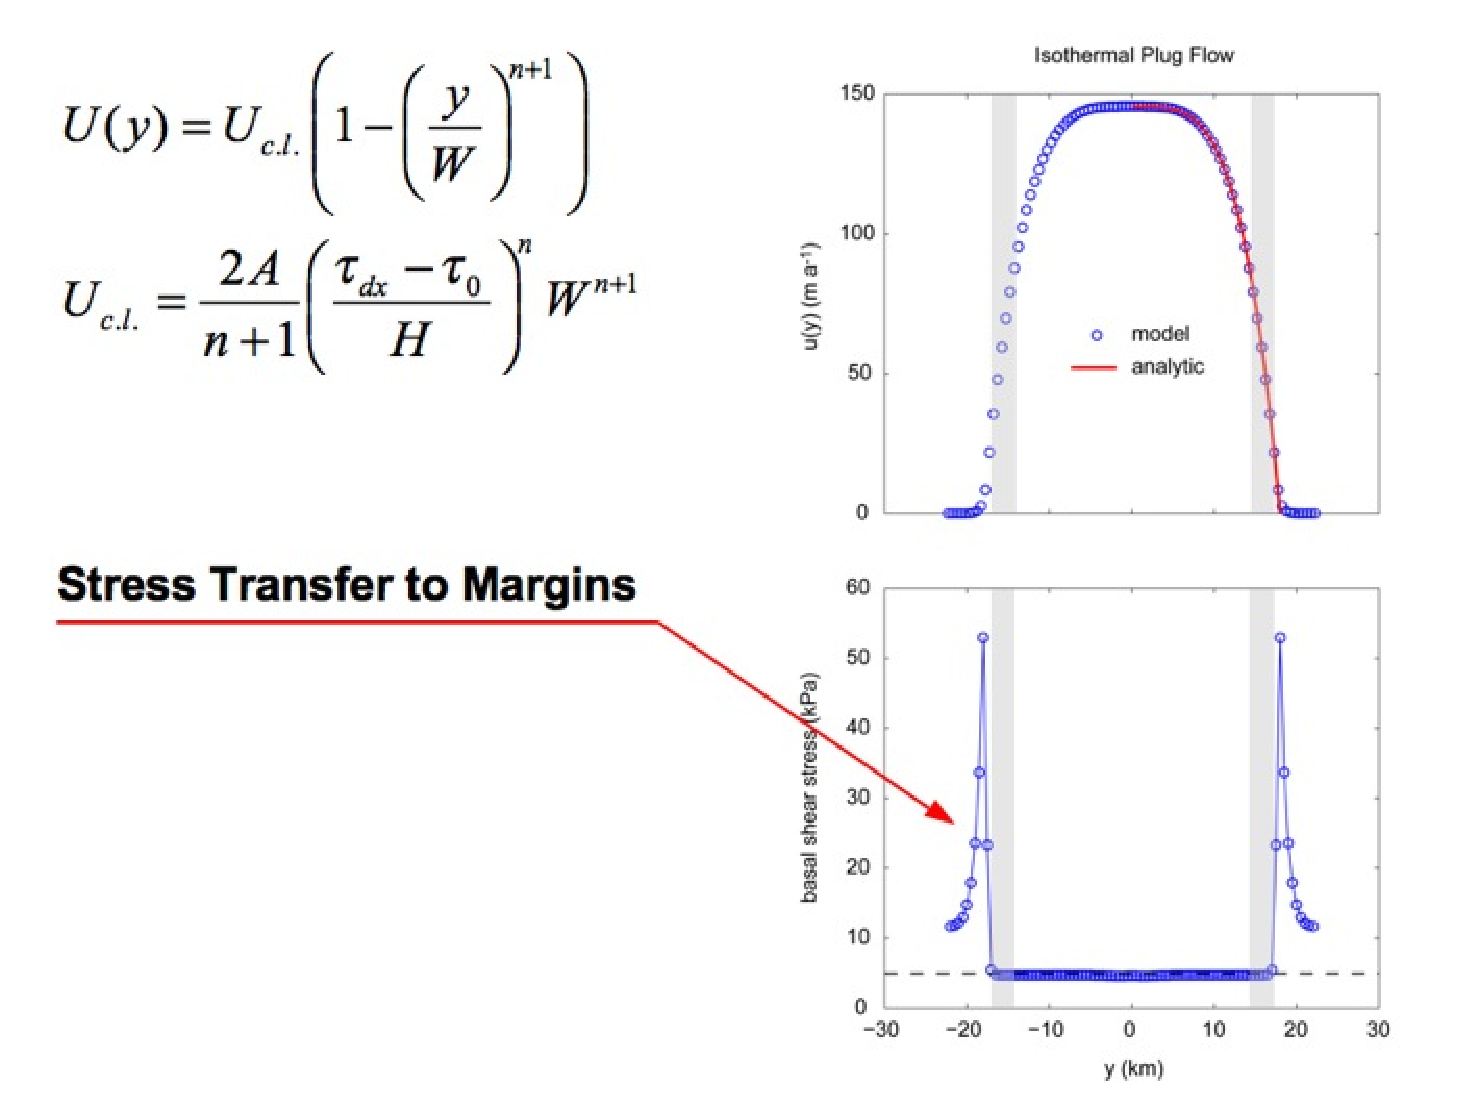
\includegraphics[width=0.65\columnwidth]{\dir/figs/Plastic_bed2.eps}
%  \end{center}
%  \caption{Across-flow profiles of velocity and basal drag from the modeled, idealized ice stream in Figure 1. In the top panel, the analytical solution from \textit{Raymond} (2005) is also shown for comparison. In the bottom panel, stress transfer to the lateral margins is clearly seen.}
%    \label{fig:plasticbed2}
%\end{figure} 

\subsection{Lateral Boundary Conditions}
Currently, the only lateral boundary condition implemented that is of any significance is that for floating ice; the depth-averaged stress resulting from an adjacent column of ocean water is applied at the location of an ice shelf (or ice tongue) front. The derivation follows largely along the lines above for the free surface and specified basal traction boundary conditions, except that the surface normal vectors, $n_{x}$ and $n_{y}$, are taken as lying entirely in the $x$, $y$ plane (that is, they are perpendicular to a vertical shelf front). Thus we have

\begin{equation}
\begin{split}
  & \hat{x}:\quad 4\eta \frac{\partial u}{\partial x}n_{x}+\eta \frac{\partial u}{\partial y}n_{y}+\eta \frac{\partial u}{\partial z}n_{z}=-2\eta \frac{\partial v}{\partial y}n_{x}-\eta \frac{\partial v}{\partial x}n_{y}+\rho g\left( s-z \right)n_{x}-S_{x}, \\ 
 & \hat{y}:\quad 4\eta \frac{\partial v}{\partial y}n_{y}+\eta \frac{\partial v}{\partial x}n_{x}+\eta \frac{\partial v}{\partial z}n_{z}=-2\eta \frac{\partial u}{\partial x}n_{y}-\eta \frac{\partial u}{\partial y}n_{x}+\rho g\left( s-z \right)n_{y}-S_{y} \\ 
\end{split}
\end{equation}

where $S_x$ and $S_y$ are source terms from the pressure due to ocean water (to be defined below) and $\rho g\left( s-z \right)$ comes from including the 1st-order vertical stress balance,

\begin{equation}
\begin{split}
  & \frac{\partial \sigma _{zz}}{\partial z}=\frac{\partial \tau _{zz}}{\partial z}-\frac{\partial P}{\partial z}=\rho g\quad \text{(integrate w}\text{.r}\text{.t}\text{. $z$)}, \\ 
 & P=\rho g\left( s-z \right)+\tau _{zz}, \\ 
 & P=\rho g\left( s-z \right)+2\eta \dot{\varepsilon }_{zz}=\rho g\left( s-z \right)+2\eta \left( -\frac{\partial u}{\partial x}-\frac{\partial v}{\partial y} \right), \\ 
\end{split}
\end{equation}

with \textit{\(\rho{}\)} being the ice density. In the last step above we have used the constitutive relation and incompressibility to expand the vertical, normal-deviatoric stress in terms of the effective viscosity and horizontal-normal strain rates. We calculate the source terms $S_x$ and $S_y$ as the depth-averaged stress at the ice shelf front due to the pressure of ocean water there. This value is given by

\begin{equation}
S_{i}=\left[ \frac{1}{H}\frac{1}{2}\rho _{w}g\left( H-h_f \right)^{2} \right]n_{i}=\left[ \frac{1}{2}\rho _{w}gH\left( \frac{\rho }{\rho _{w}} \right)^{2} \right]n_{i},\quad \quad h_f=H\left( 1-\frac{\rho _{{}}}{\rho _{w}} \right),
\end{equation}

where  \textit{i=x,y}, $n_i$ is the shelf-front normal vector, $H$ is the ice thickness, $h_f$ is the ``freeboard'', or ice thickness above floatation, and $\rho_w$ is the density of ocean water. Because we have taken a depth-average for this source term, we take a depth-average of the term $\rho g\left( s-z \right)$ above, which is $\frac{1}{2}\rho gH$.

Combining these two terms and inserting them in the horizontal boundary condition expressions above gives

\begin{equation}
\begin{split}
& \hat{x}:\quad 4\eta \frac{\partial u}{\partial x}n_{x}+\eta \frac{\partial u}{\partial y}n_{y}+\eta \frac{\partial u}{\partial z}n_{z}= \\
& -2\eta \frac{\partial v}{\partial y}n_{x}-\eta \frac{\partial v}{\partial x}n_{y}+\left[ -\frac{1}{2}H\left( \frac{\rho }{\rho _{w}} \right)^{2}\rho _{w}g+\frac{1}{2}\rho gH \right]n_{x}, \\ 
 & \hat{y}:\quad 4\eta \frac{\partial v}{\partial y}n_{y}+\eta \frac{\partial v}{\partial x}n_{x}+\eta \frac{\partial v}{\partial z}n_{z}= \\
 & -2\eta \frac{\partial u}{\partial x}n_{y}-\eta \frac{\partial u}{\partial y}n_{x}+\left[ -\frac{1}{2}H\left( \frac{\rho }{\rho _{w}} \right)^{2}\rho _{w}g+\frac{1}{2}\rho gH \right]n_{y}, \\ 
\end{split}
\end{equation}

which can be rearranged to

\begin{equation}
\begin{split}
  & \hat{x}:\quad 4\frac{\partial u}{\partial x}n_{x}+\frac{\partial u}{\partial y}n_{y}+\frac{\partial u}{\partial z}n_{z}+2\frac{\partial v}{\partial y}n_{x}+\frac{\partial v}{\partial x}n_{y}=\frac{\rho gH}{2\eta }\left( 1-\frac{\rho }{\rho _{w}} \right)n_{x}, \\ 
 & \hat{y}:\quad 4\frac{\partial v}{\partial y}n_{y}+\frac{\partial v}{\partial x}n_{x}+\frac{\partial v}{\partial z}n_{z}+2\frac{\partial u}{\partial x}n_{y}+\frac{\partial u}{\partial y}n_{x}=\frac{\rho gH}{2\eta }\left( 1-\frac{\rho }{\rho _{w}} \right)n_{y}. \\ 
\end{split}
\end{equation}

For an ice shelf, the surface and basal velocities are equal, in which case the vertical velocity gradient terms are $\sim{0}$, giving the final form of the lateral boundary conditions implemented in the model,

\begin{equation}
\begin{split}
  & \hat{x}:\quad 4\frac{\partial u}{\partial x}n_{x}+\frac{\partial u}{\partial y}n_{y}+2\frac{\partial v}{\partial y}n_{x}+\frac{\partial v}{\partial x}n_{y}=\frac{\rho gH}{2\eta }\left( 1-\frac{\rho }{\rho _{w}} \right)n_{x}, \\ 
 & \hat{y}:\quad 4\frac{\partial v}{\partial y}n_{y}+\frac{\partial v}{\partial x}n_{x}+2\frac{\partial u}{\partial x}n_{y}+\frac{\partial u}{\partial y}n_{x}=\frac{\rho gH}{2\eta }\left( 1-\frac{\rho }{\rho _{w}} \right)n_{y}. \\ 
\end{split}
\end{equation}

\subsection{Summary}
Note that the form for \textit{all} of the boundary conditions above is very similar. In fact, all that differs among the equations for the free surface, the specified basal traction, and the lateral shelf boundary condition is (1) the definition of the normal vectors and (2) the existence and definition of a source term. Here are the \textit{x} direction equations again for the three cases:

\begin{equation}
\begin{split}
  & \hat{x}:\quad 4\frac{\partial u}{\partial x}\frac{\partial s}{\partial x}+ \frac{\partial u}{\partial y}\frac{\partial s}{\partial y}+2 \frac{\partial v}{\partial y}\frac{\partial s}{\partial x}+\frac{\partial v}{\partial x}\frac{\partial s}{\partial y}-\frac{\partial u}{\partial z}=0, \\ 
  & \hat{x}:\quad 4\frac{\partial u}{\partial x}\frac{\partial b}{\partial x}+\frac{\partial u}{\partial y}\frac{\partial b}{\partial y}+2\frac{\partial v}{\partial y}\frac{\partial b}{\partial x}+\frac{\partial v}{\partial x}\frac{\partial b}{\partial y}-\frac{\partial u}{\partial z}=\frac{\tau _{bx}}{\eta }, \\ 
  & \hat{x}:\quad 4\frac{\partial u}{\partial x}n_{x}+\frac{\partial u}{\partial y}n_{y}+2\frac{\partial v}{\partial y}n_{x}+\frac{\partial v}{\partial x}n_{y}=\frac{\rho gH}{2\eta }\left( 1-\frac{\rho }{\rho _{w}} \right)n_{x}. \\
\end{split}
\end{equation}

In the first equation (free surface), the normals are related to the ice sheet surface slope and the source term is zero (which subsequently allows us to divide through by the effective viscosity and remove it from the equations). In the second equation (specified basal traction), the normals are related to the bedrock slopes and the source term is related to the assumed relationship between the basal shear stress and the basal sliding rate. In the last equation, the normals are defined by the shape of the ice-shelf front in map view, the vertical velocity gradient terms are absent, and the source term is related to the pressure from the adjacent column of ocean water.


\section{Numerical Solution of Higher-Order Equations}

\textbf{SP: Note that this will have to be updated by Bill at some point. We might be able to get away with some of what is in here for the short term.}

\subsection{Governing Equations}
The final form of the equations we'd like to solve is:
 
\begin{align*}
 & x: \quad 4\frac{\partial }{\partial x}\left( \eta \frac{\partial u}{\partial x} \right)+\frac{\partial }{\partial y}\left( \eta \frac{\partial u}{\partial y} \right)+\frac{\partial }{\partial z}\left( \eta \frac{\partial u}{\partial z} \right)= \\
 &-2\frac{\partial }{\partial x}\left( \eta \frac{\partial v}{\partial y} \right)-\frac{\partial }{\partial y}\left( \eta \frac{\partial v}{\partial x} \right)+\rho g\frac{\partial s}{\partial x} \\ 
 & y: \quad 4\frac{\partial }{\partial y}\left( \eta \frac{\partial v}{\partial y} \right)+\frac{\partial }{\partial x}\left( \eta \frac{\partial v}{\partial x} \right)+\frac{\partial }{\partial z}\left( \eta \frac{\partial v}{\partial z} \right)= \\
 & -2\frac{\partial }{\partial y}\left( \eta \frac{\partial u}{\partial x} \right)-\frac{\partial }{\partial x}\left( \eta \frac{\partial u}{\partial y} \right)+\rho g\frac{\partial s}{\partial y} \\ 
\end{align*}

\subsection{Coordinate Transform}
For ice sheet modeling, it is convenient to recast the governing equations using a dimensionless, stretched vertical coordinate (often called a sigma coordinates). The stretched vertical coordinate is defined as:

\begin{align*}
\sigma = \frac{(s - z)}{H}.
\end{align*}

This means that at the surface of the ice sheet $\sigma = 0$, and at the base $\sigma = 1$ regardless of the ice thickness.  As a result of this transformation, a coordinate ($x,y,z$) is mapped to ($x',y',\sigma$).  This means that function derivatives must be re-written (using $\frac{\partial f}{\partial x}$ as an example) as:

\begin{align*}
\frac{\partial f}{\partial x} = \frac{\partial f}{\partial x'} \frac{\partial x'}{\partial x} + \frac{\partial f}{\partial y'} \frac{\partial y'}{\partial x} + \frac{\partial f}{\partial \sigma} \frac{\partial \sigma}{\partial x}.
\end{align*}

Similarly for $\frac{\partial f}{\partial y}$ and $\frac{\partial f}{\partial z}$. We can simplify this by assuming that 

\begin{align*}
\frac{\partial x'}{\partial x}, \frac{\partial y'}{\partial y} = 1
\end{align*}

and

\begin{align*}
\frac{\partial x'}{\partial y}, \frac{\partial x'}{\partial z}, \frac{\partial y'}{\partial x}, \frac{\partial y'}{\partial z} = 0,
\end{align*}

which is valid if the bed and surface gradients are not too large. This simplifies the above to:

\begin{align*}
\frac{\partial f}{\partial x} = \frac{\partial f}{\partial x'} + \frac{\partial f}{\partial \sigma}\frac{\partial \sigma}{\partial x},
\end{align*}

\begin{align*}
\frac{\partial f}{\partial y} = \frac{\partial f}{\partial y'} + \frac{\partial f}{\partial \sigma}\frac{\partial \sigma}{\partial y},
\end{align*}

\begin{align*}
\frac{\partial f}{\partial z} = \frac{\partial f}{\partial \sigma}\frac{\partial \sigma}{\partial z}.
\end{align*}

Rescaling parameters $a_{x}$, $a_{y}$, $b_{x}$, $b_{y}$, and $c_{xy}$ are defined. For the $x$ derivative case (the $y$ derivative case is analogous) we have

\begin{align*}
a_{x} = \frac{1}{H}(\frac{\partial s}{\partial x'} - \sigma \frac{\partial H}{\partial x'}),
\end{align*}

\begin{align*}
b_{x} = \frac{\partial a_x}{\partial x'} + a_x \frac{\partial a_x}{\partial \sigma} 
    = \frac{1}{H} (\frac{\partial^2 s}{\partial x'^2} - \sigma \frac{\partial^2 H}{\partial x'^2} - 2a_x \frac{\partial H}{\partial x'}),
\end{align*}

\begin{align*}
c_{xy} = \frac{\partial a_y}{\partial x'} + a_x \frac{\partial a_y}{\partial \sigma} 
       = \frac{\partial a_x}{\partial y'} + a_y \frac{\partial a_x}{\partial \sigma}.
\end{align*}

Using these, expressions for the $x$ derivatives become:

\begin{align*}
\frac{\partial f}{\partial x} = \frac{\partial f}{\partial x'} + a_x \frac{\partial f}{\partial \sigma},
\end{align*}

\begin{align*}
 & \frac{\partial }{\partial x}\left( \eta \frac{\partial u}{\partial x} \right)=\frac{\partial }{\partial \hat{x}}\left( \eta \frac{\partial u}{\partial \hat{x}} \right)+\frac{\partial \sigma }{\partial \hat{x}}\frac{\partial }{\partial \sigma }\left( \eta \frac{\partial u}{\partial \hat{x}} \right)+\frac{\partial \sigma }{\partial \hat{x}}\frac{\partial }{\partial \hat{x}}\left( \eta \frac{\partial u}{\partial \sigma } \right)+ \\
& \left( \frac{\partial \sigma }{\partial \hat{x}} \right)^{2}\frac{\partial }{\partial \sigma }\left( \eta \frac{\partial u}{\partial \sigma } \right)+\left( \frac{\partial _{{}}^{2}\sigma }{\partial \hat{x}_{{}}^{2}} \right)\eta \frac{\partial u}{\partial \sigma }
\end{align*}

where hatted values refer to the coordinate directions in sigma coordinates. Similarly, the first cross-stress term on the RHS is given by

\begin{align*}
&\frac{\partial }{\partial x}\left( \eta \frac{\partial v}{\partial y} \right)=\frac{\partial }{\partial \hat{x}}\left( \eta \frac{\partial v}{\partial \hat{y}} \right)\,+\frac{\partial \sigma }{\partial \hat{x}}\frac{\partial }{\partial \sigma }\left( \eta \frac{\partial v}{\partial \hat{y}} \right)\,+\frac{\partial \sigma }{\partial \hat{y}}\frac{\partial }{\partial \hat{x}}\left( \eta \frac{\partial v}{\partial \sigma } \right)\,+ \\
&\frac{\partial \sigma }{\partial \hat{x}}\frac{\partial \sigma }{\partial \hat{y}}\frac{\partial }{\partial \sigma }\left( \eta \frac{\partial v}{\partial \sigma } \right)\,+\frac{\partial _{{}}^{2}\sigma }{\partial \hat{x}\partial \hat{y}}\eta \frac{\partial v}{\partial \sigma }\,
\end{align*}


One term has become five terms and each one of those is pretty ugly looking on its own. Luckily, there is a lot of symmetry here. Notice that if we wanted to design subroutines to discretize the terms on the RHS, we could re-use a lot of them by either applying them to the correct velocity component (to either the $u$ or the $v$ discretization) or by passing the appropriate arguments (by passing either the grid spacing in the $x$ direction or the $y$ direction, where appropriate).

A similar transform is applied to each of the terms in the governing equations given above. At any point within the grid, the grid spacing, coordinate transform, and viscosity information associated with the unknown velocity components is made discrete using finite differences. This information ultimately equates to coefficients on the unknown velocities, allowing the governing equations over the entire grid (with appropriate discretizations for boundary conditions) to be recast as a system of $n$ equations in $n$ unknowns. In turn, this system is solved using standard linear algebraic methods for large, sparse systems of linear equations.

\subsection{Operating Splitting}
In the governing equations given above, note that for the \textit{x} equation we have moved all terms containing gradients in \textit{v} to the right-hand side (RHS) (and vice-versa for the \textit{y} equation). 

This allows us to solve the equations using an $operator$ $splitting$ approach; for the $x$ equation, we treat $v$ as known (where we take the values of $v$ from the previous iteration, as discussed further below) and solve for $u$, and vice versa when we solve the $y$ equation for $v$. The splitting refers to the fact that we are breaking the multi-dimensional divergence operation into two steps; rather than solving one big matrix equation for $u$ and $v$ simultaneously, we solve two smaller matrix equations in sequence with one of the unknowns treated as a known source term on the RHS of the equation. This procedure was probably more common and important years ago when it was desirable to keep the matrix equations as small as possible for memory management issues. On today's machines, with fewer memory limitations (in particular when dealing with codes designed to run on parallel, distributed memory architectures) this splitting is not necessary and may even lead to some undesirable numerical side effects (i.e. a slow-down in the convergence of iterations used to treat nonlinearity in the governing equations).

A general matrix form of the split equations, where coefficients on the $u$ and $v$ velocity components (i.e. viscosity, grid spacing, scalars) are contained in the block matrices \textbf{A}, is given by 

\begin{align*}
\begin{matrix}
  \left[ \begin{matrix}
   \mathbf{A}_{\mathbf{uu}} & \mathbf{0}  \\
   \mathbf{0} & \mathbf{A}_{\mathbf{vv}}  \\
\end{matrix} \right]\left[ \begin{matrix}
   \mathbf{u}  \\
   \mathbf{v}  \\
\end{matrix} \right]=\left[ \begin{matrix}
   \mathbf{b}_{\mathbf{u}}-\mathbf{A}_{\mathbf{uv}}\mathbf{v}  \\
   \mathbf{b}_{\mathbf{v}}-\mathbf{A}_{\mathbf{vu}}\mathbf{u}  \\
\end{matrix} \right] \\ 
   \\ 
  \mathbf{A}_{\mathbf{uu}}\mathbf{u}=\mathbf{b}_{\mathbf{u}}-\mathbf{A}_{\mathbf{uv}}\mathbf{v},\quad \quad \mathbf{A}_{\mathbf{vv}}\mathbf{v}=\mathbf{b}_{\mathbf{v}}-\mathbf{A}_{\mathbf{vu}}\mathbf{u} \\ 
\end{matrix}
\end{align*}

where the \textbf{uu} subscript denotes block matrices containing coefficients for gradients on \textit{u} in the equation for the \textit{x} component of velocity (i.e. \textit{u}). The subscript \textbf{uv} denotes block matrices containing coefficients for gradients on \textit{v} in the equation for the \textit{x} component of velocity (and similarly for the \textbf{vv} and \textbf{vu} subscripts). On the right-hand side, the single subscripts \textbf{u} and \textbf{v} are attached to the geometric source terms for the \textit{x} and \textit{y} components of velocity, respectively.

\subsection{Solution of the Non-linear System Through a Fixed Point Iteration}
The non-linearity in the equations -- the fact that the coefficients on the velocity components (the viscosity) are dependent on the velocity (or more specifically, the velocity gradients) -- is handled through a fixed-point iteration. A general fixed point iteration for a vector of unknowns \textit{u} can be written as 

\begin{align*}
u^{k}=\mathbf{B}\left( u^{k-1} \right),
\end{align*}

where \textit{k} is the index for the \textit{u} being solved for and \textbf{B} is a matrix operation performed on the components of \textit{u} obtained at the previous iteration, \textit{k-1}. The fixed point occurs when the values of \textit{u} at \textit{k} and \textit{k-1} are equal to within some given tolerance (at which point the iteration process is halted). CISM has options for implementing both Picard and Newton-based fixed-point iterations. For the Picard iteration (standard in CISM), the matrix coefficients with a velocity dependence are simply based on the velocities obtained at the previous iteration. In most cases, this equates to using velocities obtained from the previous iteration to calculate the strain rate components that go into the calculation of the effective viscosity, $\eta$.

\section{Final Matrix Form}
When accounting for both the operator splitting and the Picard iteration on the effective viscosity, the final form of the matrix equations solved in CISM becomes 

\begin{align*}
\begin{matrix}
  \left[ \begin{matrix}
   \mathbf{A}_{\mathbf{uu}}^{k-1} & \mathbf{0}  \\
   \mathbf{0} & \mathbf{A}_{\mathbf{vv}}^{k-1}  \\
\end{matrix} \right]\left[ \begin{matrix}
   \mathbf{u}^{k}  \\
   \mathbf{v}^{k}  \\
\end{matrix} \right]=\left[ \begin{matrix}
   \mathbf{b}_{\mathbf{u}}-\mathbf{A}_{\mathbf{uv}}^{k-1}\mathbf{v}^{k-1}  \\
   \mathbf{b}_{\mathbf{v}}-\mathbf{A}_{\mathbf{vu}}^{k-1}\mathbf{u}^{k-1}  \\
\end{matrix} \right] \\ 
   \\ 
  \mathbf{A}_{\mathbf{uu}}^{k-1}\mathbf{u}=\mathbf{b}_{\mathbf{u}}-\mathbf{A}_{\mathbf{uv}}^{k-1}\mathbf{v}^{k-1},\quad \quad \mathbf{A}_{\mathbf{vv}}^{k-1}\mathbf{v}=\mathbf{b}_{\mathbf{v}}-\mathbf{A}_{\mathbf{vu}}^{k-1}\mathbf{u}^{k-1} \\ 
\end{matrix}
\end{align*}

where the index \textit{k} denotes an unknown value being solved for during the current non-linear iteration and the index \textit{k}-1 denotes a lagged value taken from solution at the end of the previous non-linear iteration (again, here the lagging is primarily with respect to the effective viscosity, the value of which is calculated using velocity gradients obtained at the end of the previous iteration). The final form of the matrix equations given above represents a linear system; for the solution at any particular nonlinear iteration \textit{k}, all of the coefficients on the unknown velocity components \textit{u} and \textit{v} are held frozen during the solution of the linear system. This linear system can be solved using any practical method. For large, sparse systems, some variant on the iterative conjugate gradient method (e.g. BiCG, GMRES) is generally the most efficient. In this case the linear system is not solved exactly but is solved to within some small tolerance of the true solution.

\subsection{Newton-based Methods for Solutions of the Non-linear System}
Without any operator splitting, the generic matrix form of the equations to be solved can be written as

\begin{align*}
\mathbf{A}(\mathbf{u})\mathbf{u}=\mathbf{b}.
\end{align*}

The linearized form of the equations to be solved using the Picard solution can be written as

\begin{align*}
\mathbf{u}^{k}=\mathbf{A}(\mathbf{u}^{k-1})^{-1}\mathbf{b}.
\end{align*}

The full nonlinear system to be solved can be written as

\begin{align*}
\mathbf{F}(\mathbf{u})=\mathbf{A}(\mathbf{u})\mathbf{u}-\mathbf{b}
\end{align*}

with the solution for the uknown vector \textit{u} given by 

\begin{align*}
\mathbf{F}(\mathbf{u})=0.
\end{align*}

A Newton-based solution for this system of equations, based on a first-order Taylor series expansion about the solution for \textit{u} at iteration \textit{k-1}, can be written as

\begin{align*}
\mathbf{F}(\mathbf{u}^{k})=\mathbf{F}(\mathbf{u}^{k-1})+\mathbf{F}(\mathbf{u}^{k-1})\delta \mathbf{u}^{k-1},
\end{align*}

where

\begin{align*}
\mathbf{F}(\mathbf{u}^{k-1})=\mathbf{J}^{k-1}
\end{align*}

is the system Jacobian with individual components give by

\begin{align*}
J_{ij}=\frac{\partial F_{i}(\mathbf{u}^{k-1})}{\partial u_{j}}
\end{align*}

and 

\begin{align*}
\delta \mathbf{u}^{k-1}=\mathbf{u}^{k}-\mathbf{u}^{k-1}
\end{align*}

is the Newton update to be solved for. One method for doing so is by solving 

\begin{align*}
\delta \mathbf{u}^{k-1}=-\left( \mathbf{J}^{k-1} \right)^{-1}\mathbf{F}(\mathbf{u}^{k-1}).
\end{align*}

The advantage of Newton-based methods is that, with a good initial guess for the solution, convergence rates are very often quadratic (e.g. the residual decreases quadratically, so that at iteration \textit{k} one has a residual of 0.1, at iteration \textit{k+1}, a residual of 0.01, and at iteration \textit{k+2} a residual of 0.0001), whereas Picard-based iterations are much slower to converge. A figure comparing rates of convergence for Picard versus Newton on a CISM tests case is shown below (Figure \ref{fig:jfnk}. The Newton method is based on the work of Lemieux et al. ($J.$ $Comput.$ $Phys.$, \textbf{230}, 2011), which is discussed further below.

%\begin{figure}
%  \begin{center}
%    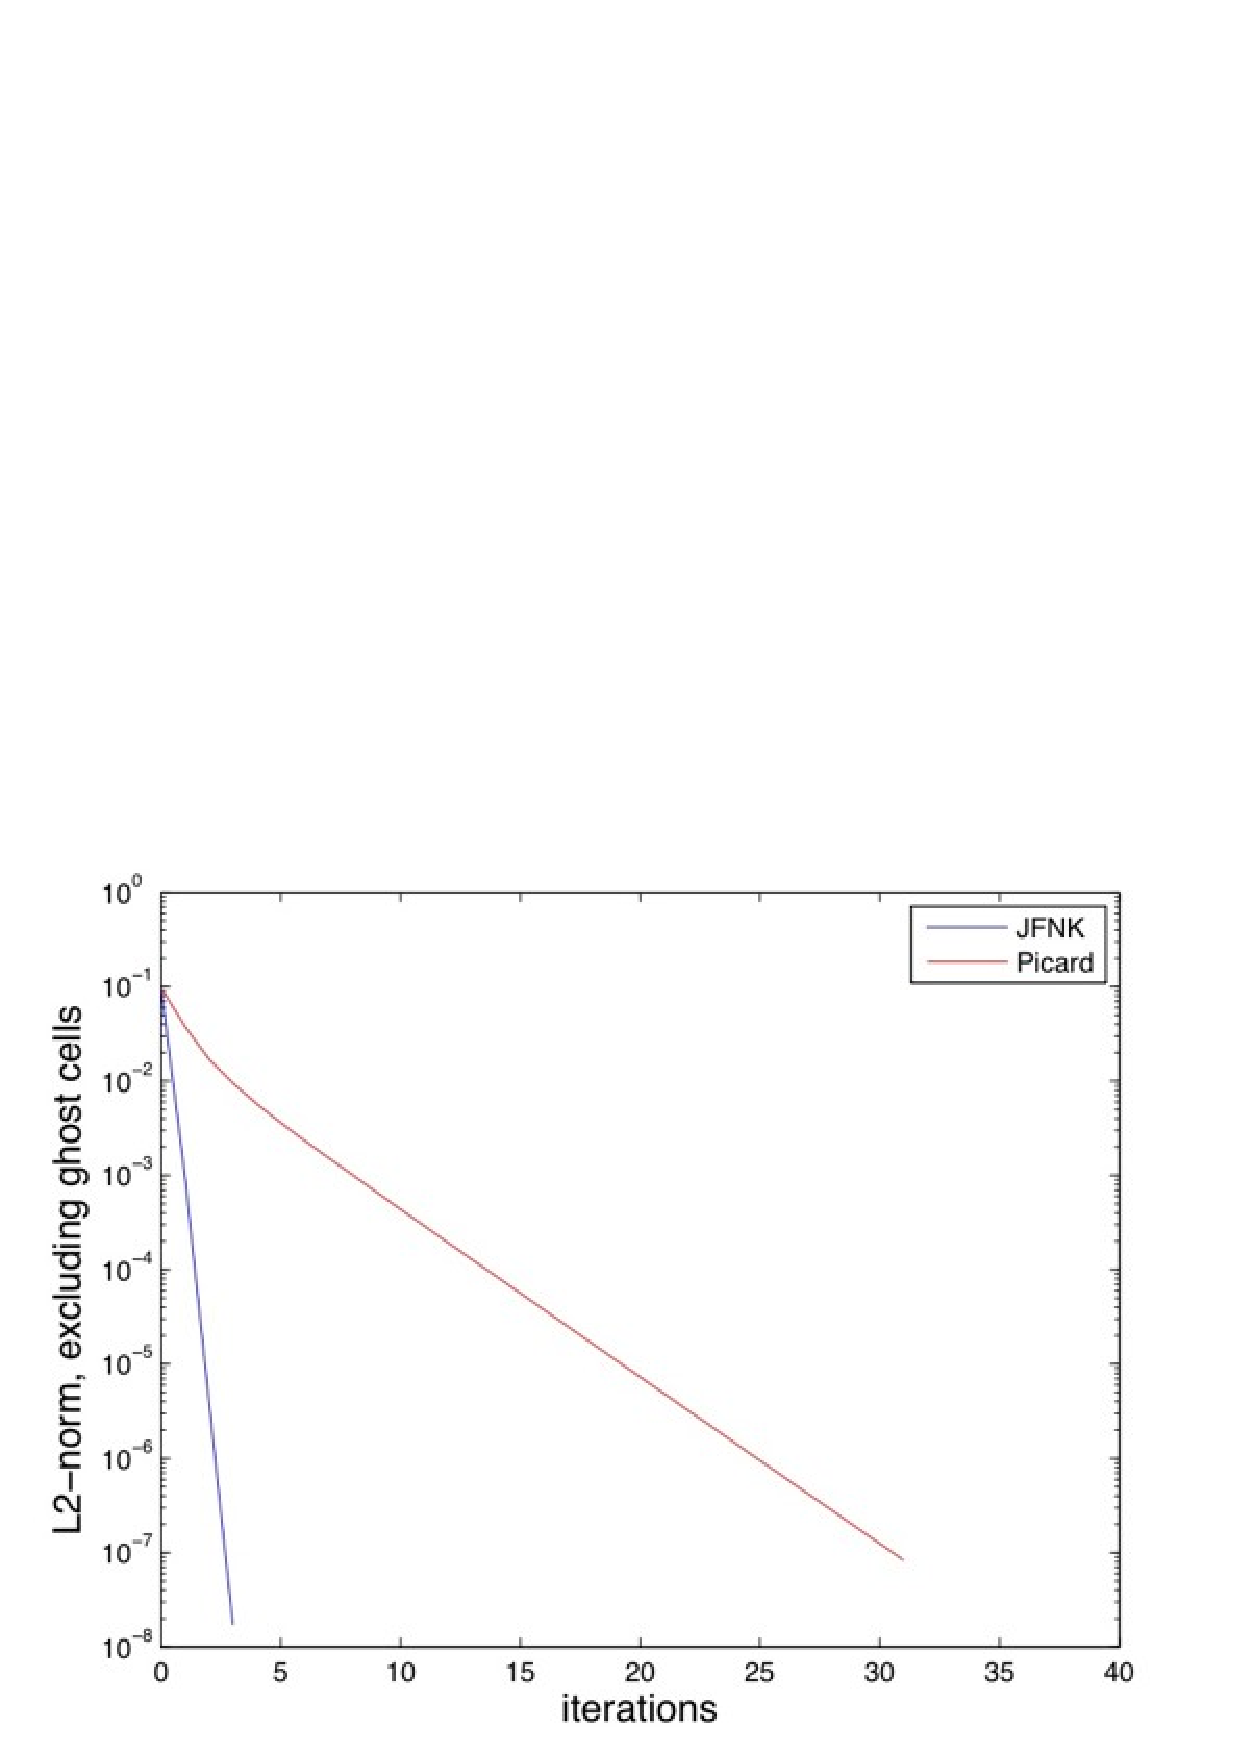
\includegraphics[width=0.9\columnwidth]{\dir/figs/Picard_vs_newton.png}
%  \end{center}
%  \caption{Rates of convergence for the nonlinear iteration in CISM.}
%  \label{fig:jfnk}
%\end{figure} 

\subsection{The Jacobian Free Approach}
In practice, the model Jacobian may either be too difficult or to expensive too form. A Jacobian Free Newton-Krylov (JFNK) approach has recently been implemented in CISM (Leimieux et al., 2011), largely following methods discussed in Knoll and Keyes ($J.$ $Comput.$ $Phys.$, \textbf{193}, 2004).

The crux of the method comes from noting that, when solving the last equation above using a Krylov method (e.g. Conjugate Gradients, GMRES, etc.) the solution for the Newton update is taken from a combination of Krylov vectors that span the subspace


\begin{align*}
span\left\{ \mathbf{r}_{0},\mathbf{Jr}_{0},\mathbf{J}^{2}\mathbf{r}_{0},...,\mathbf{J}^{n-1}\mathbf{r}_{0} \right\}=span\left\{ \mathbf{r}_{0},\mathbf{Jv}_{1},\mathbf{Jv}_{2},...,\mathbf{Jv}_{n-1} \right\}.
\end{align*}

This implies that, when using a Krylov method, one only ever needs to calculate matrix vector products of the form $\mathbf{Jv}$ when building up the subspace that approximates the solution vector $\delta \mathbf{u}$.

Following Knoll and Keyes (2004), note that the necessary matrix vector products can be approximated through nonlinear function evaluations and a perturbation as

\begin{align*}
\mathbf{Jv}\approx \frac{\mathbf{F}\left( \mathbf{u}+\varepsilon \mathbf{v} \right)-\mathbf{F}\left( \mathbf{u} \right)}{\varepsilon }.
\end{align*}

It is not immediately obvious why this approximation is valid. To verify this, take a few steps back and consider a nonlinear system of equations of two variables, $u_{1}$ and $u_{2}$. The right-hand side of the above equation can be expanded as

\begin{align*}
\frac{\mathbf{F}\left( \mathbf{u}+\varepsilon \mathbf{v} \right)-\mathbf{F}\left( \mathbf{u} \right)}{\varepsilon }=\left[ \begin{matrix}
   \frac{F_{1}\left( u_{1}+\varepsilon v_{1},u_{2}+\varepsilon v_{2} \right)-F_{1}(u_{1},u_{2})}{\varepsilon }  \\
   \frac{F_{2}\left( u_{1}+\varepsilon v_{1},u_{2}+\varepsilon v_{2} \right)-F_{2}(u_{1},u_{2})}{\varepsilon }  \\
\end{matrix} \right].
\end{align*}

A first-order Taylor series expansion approximation to this is given by

\begin{align*}
\frac{\mathbf{F}\left( \mathbf{u}+\varepsilon \mathbf{v} \right)-\mathbf{F}\left( \mathbf{u} \right)}{\varepsilon }\approx \left[ \begin{matrix}
   \frac{F_{1}\left( u_{1},u_{2} \right)+\varepsilon v_{1}\frac{\partial F_{1}}{\partial u_{1}}+\varepsilon v_{2}\frac{\partial F_{1}}{\partial u_{2}}-F_{1}(u_{1},u_{2})}{\varepsilon }  \\
   \frac{F_{2}\left( u_{1},u_{2} \right)+\varepsilon v_{1}\frac{\partial F_{2}}{\partial u_{1}}+\varepsilon v_{2}\frac{\partial F_{2}}{\partial u_{2}}-F_{2}(u_{1},u_{2})}{\varepsilon }  \\
\end{matrix} \right],
\end{align*}

which collapses to

\begin{align*}
\frac{\mathbf{F}\left( \mathbf{u}+\varepsilon \mathbf{v} \right)-\mathbf{F}\left( \mathbf{u} \right)}{\varepsilon }\approx\left[ \begin{matrix}
   v_{1}\frac{\partial F_{1}}{\partial u_{1}}+v_{2}\frac{\partial F_{1}}{\partial u_{2}}  \\
   v_{1}\frac{\partial F_{2}}{\partial u_{1}}+v_{2}\frac{\partial F_{2}}{\partial u_{2}}  \\
\end{matrix} \right].
\end{align*}

Finally, note that the right-hand side of the above equation is equal to 

\begin{align*}
\mathbf{Jv}\approx\left[ \begin{matrix}
   v_{1}\frac{\partial F_{1}}{\partial u_{1}}+v_{2}\frac{\partial F_{1}}{\partial u_{2}}  \\
   v_{1}\frac{\partial F_{2}}{\partial u_{1}}+v_{2}\frac{\partial F_{2}}{\partial u_{2}}  \\
\end{matrix} \right],
\end{align*}

with the Jacobian matrix given by

\begin{align*}
\mathbf{J}=\left[ \begin{matrix}
   \frac{\partial F_{1}}{\partial u_{1}} & \frac{\partial F_{1}}{\partial u_{2}}  \\
   \frac{\partial F_{2}}{\partial u_{1}} & \frac{\partial F_{2}}{\partial u_{2}}  \\
\end{matrix} \right].
\end{align*}

The matrix vector product \textbf{Jv} is what needs to be calculated repeatedly while building up the Krylov subspace vectors that combine to approximate the Newton update vector $\delta \mathbf{u}$.

The important point is that at no point in this process does one need to calculate the entire Jacobian matrix. Another important point is that the accuracy of the approximation to the Jacobian is proportional to the small perturbation term, $\varepsilon$.

%\section{References}
%\begin{itemize}
%\item  {Knoll, D.A. and D.E. Keyes. Jacobian-free Newton-Krylov methods: a survey of approaches and applications, \textbf{193}, 357-397, 2004}.
%\end{itemize}
%
%\begin{itemize}
%\item  {Lemieux, J.F., S.F. Price, K.J. Evans, D. Knoll, A.G. Salinger, D. Holland, and A.J. Payne. Implementation of the Jacobian-Free Newton-Krylov method for solving the first-order ice sheet momentum balance, \textit{J. Comput. Phys.}, \textbf{230}, 6531-6545, doi:10.1016/j.jcp.2011.04.037, 2011}.
%\end{itemize}
%
%\end{document}

\section{Thickness Evolution in Higher-Order Models}
\label{sc:ho-thickness-evol}

\subsection{Conservation of mass}
As mentioned previously, conservation of mass for an ice sheet can be expressed by

\begin{align*}
\frac{\partial H}{\partial t}=-\nabla \cdot \left( \vec{U}H \right)+\dot{b},
\end{align*}

where $\vec{U}=(U,V)$ is the 2-dimensional, depth-integrated velocity vector, $H$ is the ice thickness, $\vec{U}H$ is the 2-dimensional ice flux vector, and $\dot{b}$ represents the sum of surface and basal mass balance terms. The change in thickness per unit time is given by the negative of the flux divergence plus a source term. 
%We can expand this a bit as,
%
%\begin{align*}\frac{\partial H}{\partial t}=-\left( \frac{\partial \left( UH \right)}{\partial x}+\frac{\partial \left( VH \right)}{\partial y} \right)+\dot{b}, \\ 
%\end{align*}
%
%where $\vec{U}$ is the depth-averaged velocity vector (in map plane), and \textit{U} and \textit{V} are the depth integrated \textit{x} and \textit{y} velocity fields, \textit{H} is the ice thickness, and $\dot{b}$ is the source term, which is the surface mass balance (>0 for accumulation and <0 for ablation). 
Note that the negative sign in front of the divergence (terms in parentheses on the right-hand side) insures sensible behavior: consider a section of the ice sheet where the thickness is nearly constant and there is no accumulation or ablation. If the velocity gradient along-flow is negative (the ice is slowing down), then we expect local thickening (left-hand side of the equation is $>0$) and vice versa (if the ice is speeding up along flow, we expect local thinning). This is the equation that needs to be solved to calculate the evolution of the ice sheet geometry.

\subsection{A diffusive approach}
For the case of a shallow-ice model, the values of $U$ and $V$ are recast in terms of ice thickness and elevation gradients, in which case the whole problem can be recast as a diffusion equation in ice thickness. In 1-dimension, the equation becomes

\begin{align*}
\frac{\partial H}{\partial t}=\frac{\partial }{\partial x}\left( D\frac{\partial h}{\partial x} \right)+\dot{b},\quad D=\frac{2A}{n+2}\left( \rho g \right)^{n}H^{n+2}\left| \frac{\partial h}{\partial x} \right|^{n-1},
\end{align*}

where $D$ is the non-linear diffusivity (because it depends on the solution to the equation, $H$), $A$ is the rate factor in Glen's flow law, $n$ is the power-law exponent, $h$ is the ice surface elevation, and $\rho$ and $g$ are the ice density and the acceleration due to gravity. Importantly, we need only local information in order to solve the above equation. If our velocity solution can not be solved locally, as in the case of higher-order models, we cannot easily use the above formulation to solve ice sheet evolution. In an attempt to use this form and retain a diffusion-solution approach to the problem (diffusion problems generally have nice numerical properties), we could try the following approach (again, in 1-dimensions only),

\begin{align*}
\frac{\partial H}{\partial t}=\frac{\partial }{\partial x}\left( D\frac{\partial h}{\partial x} \right)+\dot{b},\quad D=UH\left( \frac{\partial h}{\partial x} \right)^{-1},
\end{align*}

where the $U$ in the expression for $D$ is the depth-integrated velocity field from the higher-order model. This is the approach initially taken by \citet{Pattyn:2003tj} in one of the first higher-order modeling studies to deal with this particular problem. Notice that ice sheet surface slope is in the denominator of the diffusivity here and, as slopes get smaller and smaller (as they tend to do in regions of fast flow like ice streams and ice shelves) the diffusivity will get larger and larger (approaching infinity as the slope goes to zero). The faster velocities in these regions appear in the numerator of the diffusivity, also making it larger. This is a severe restriction on this approach because, for explicit schemes, the diffusive CFL condition requires that

\begin{align*}
\Delta t<\frac{\left( \Delta x \right)^{2}}{2D},
\end{align*}

where $\Delta t$ is the time step required for numerical stability and $\Delta x$ is the grid spacing. As the diffusivity goes to infinity (i.e., for faster flows and shallower slopes), the stable time step goes to zero. Thus in practice, this approach has proven very difficult to use for calculating ice sheet evolution in most of the dynamically interesting areas of ice sheets that we are interested in. An alternate approach is needed.

\subsection{Advection schemes}
An alternate approach is to solve the evolution equation using an advection scheme. Numerically, advection schemes can be more problematic than diffusion schemes, but in some cases like this one, they are difficult to avoid. The most general advection scheme is a first-order, upwind-advection scheme (as above, ``first-order" here refers to first-order accurate), and we will outline the implementation of such a scheme below.

Most ice sheet models (and fluid dynamics models in general) perform calculations on a ``staggered" grid of the type shown below in Figure \ref{fig:stag_c_grid}, where velocity components live on one grid and scalar components (e.g. temperatures, pressures, thickness, etc.) live on a grid that is staggered by 1/2 grid space in the horizontal dimensions (this is essential for numerical stability reasons that we won't discuss here).

\begin{figure}
  \begin{center}
    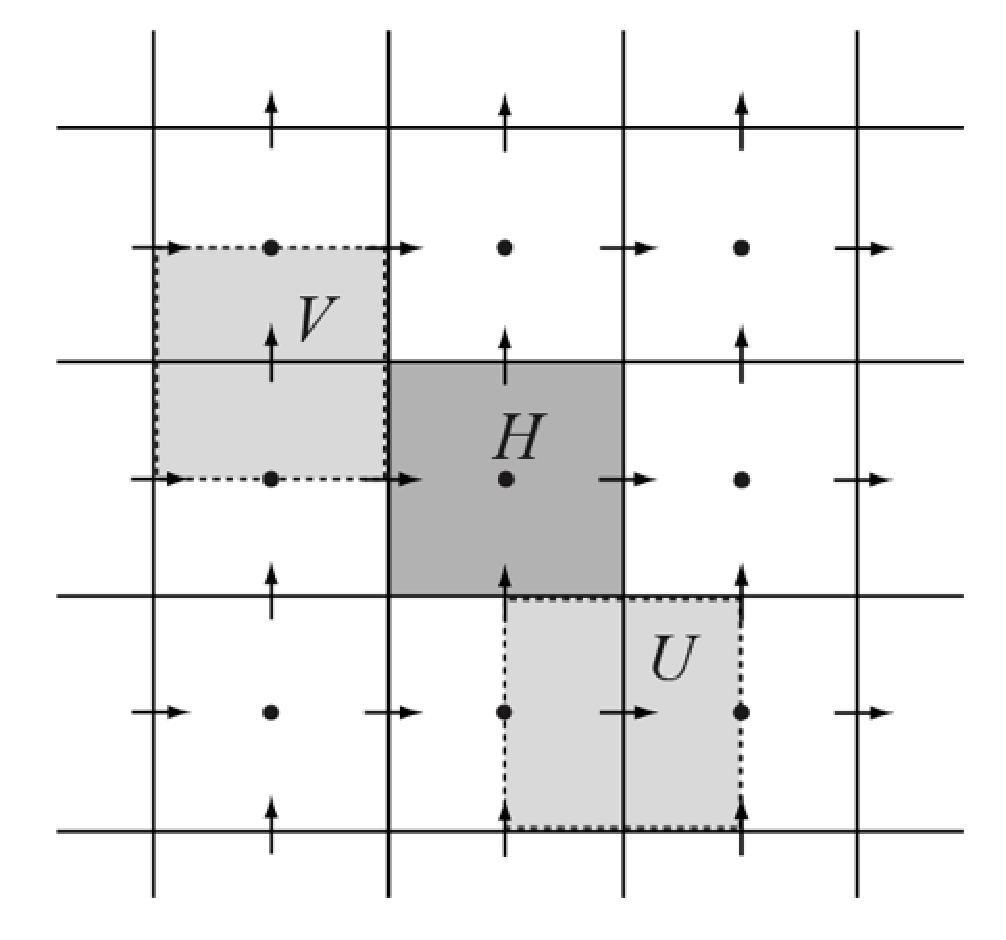
\includegraphics[width=0.4\columnwidth]{\dir/figs/Stag_grid.eps}
  \end{center}
\caption{Staggered grid in two dimensions, showing scalars (like thickness, $H$) at grid cell centers and velocity components, $U$ and $V$, at grid cell faces. This is a ``C" grid. Another staggered-grid possibility is a ``B" grid, for which both velocity components live at the grid cell corners. While CISM uses a B grid, averaging of corner velocities to face centers allows one to express them on a C grid, if necessary.}
  \label{fig:stag_c_grid}
\end{figure} 

A control volume (or finite volume) approach to solving the equation 

\begin{align*}
\frac{\partial H}{\partial t}=-\left( \frac{\partial \left( UH \right)}{\partial x}+\frac{\partial \left( VH \right)}{\partial y} \right)+\dot{b} \\ 
\end{align*}

would be to integrate our equation over a control volume centered on the scalar values (Figures \ref{fig:stag_c_grid} and \ref{fig:stag_c_grid2}). Ignoring source terms for now (assume $\dot{b}=0$), and assuming flow along the \textit{x} direction only (assume $V=0$) we have

\begin{align*}
\frac{\partial H}{\partial t}=-\frac{1}{\Delta y\Delta x}\int_{s}^{n}{\int_{w}^{e}{\frac{\partial \left( UH \right)}{\partial x}}}dxdy=-\frac{1}{\Delta y\Delta x}\left( HU_{e}-HU_{w} \right)\Delta y. \\
\end{align*}

The ``east" and ``west" (subscripts $e$ and $w$) faces of the control volume are shown in Figure \ref{fig:stag_c_grid2}.

\begin{figure}
  \begin{center}
    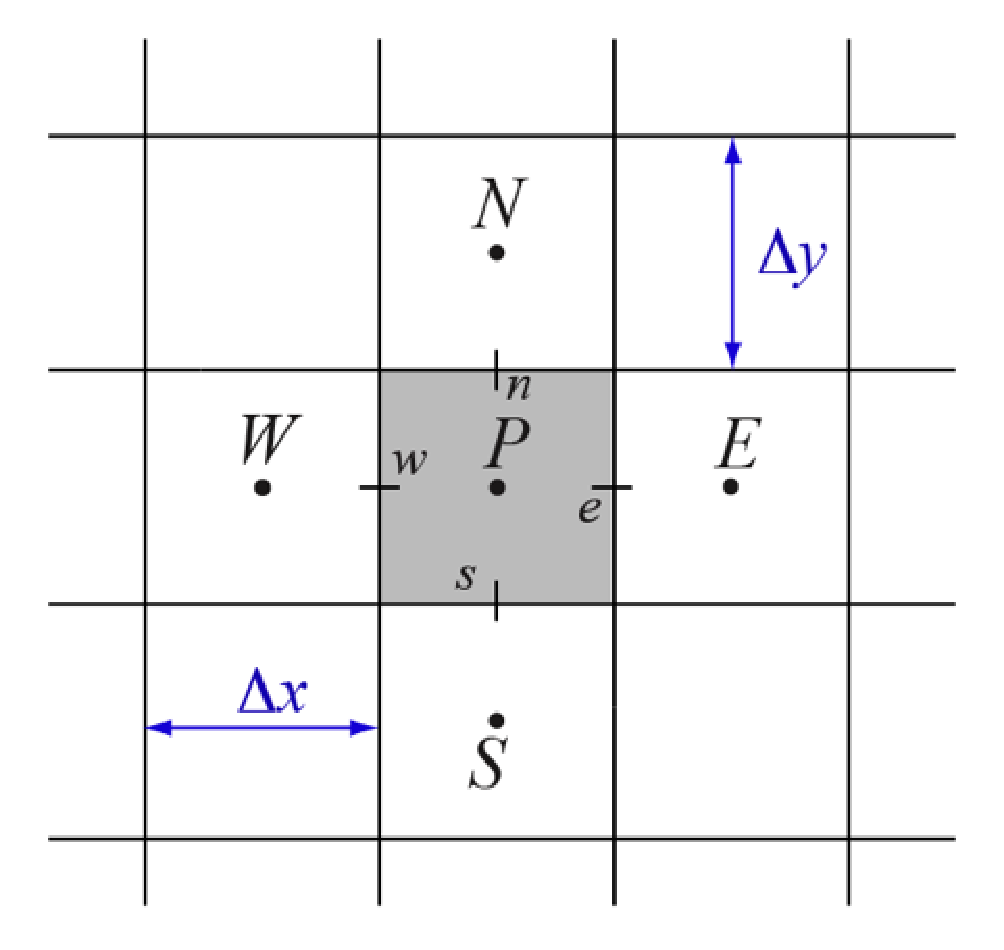
\includegraphics[width=0.4\columnwidth]{\dir/figs/Stag_gridb.eps}
  \end{center}
  \caption{Staggered grid in two dimensions, showing locations of interfaces and control volume dimensions. Interfaces \textit{e}, \textit{w}, \textit{n} and \textit{s} connect the volume centered at \textit{P} with those volumes to the east, west, north, and south (\textit{E}, \textit{W}, \textit{N}, and \textit{S}).}
  \label{fig:stag_c_grid2}
\end{figure} 

In the above equation, we have deliberately left it vague as to which value of $H$ is being advected across the east and west interfaces, into or out of the volume. This is where the term ``upwinding" comes in -- we choose the scalar value to advect across the interface based on an upwinding criterion. If, for example, the flow at interface $e$ is from left to right ($U>0$), we would advect the value of $H$ at $P$ \textit{out} of the volume centered at $P$ and \textit{into} the volume centered at $E$. If, on the other hand, the flow at $e$ was from right to left ($U<0$), we would advect the value of $H$ at $E$ \textit{into} the volume at $P$ and \textit{out} of the volume at $E$. 

The product of velocity, thickness, and the grid spacing at each interface gives a volume flux in units of cubic meters per year. The sum of the volume fluxes over the total number of faces being considered (two in this case, but four for the 2-dimensional case) gives the total volume flux in (total$>$0) or out (total$<$0) of the volume. When this number is divided by the area of the volume, the result is the mean thickness change in that volume, per unit time, that is required to maintain conservation of mass.

\subsection{Explicit vs. Implicit Evolution Schemes}

Is this an explicit or implicit scheme? If we discretize the right-hand side of the primary equation in time we get

\begin{align*}
  & \frac{\partial H}{\partial t}=-\nabla \cdot \left( UH \right)+\dot{b}, \\
 & \frac{H_{t=1}-H_{t=0}}{\Delta t}\approx -\nabla \cdot \left( UH \right)+\dot{b}.\\
\end{align*}

This can be rearranged to,

\begin{align*}
H_{t_{t=1}}\approx H_{t=0}+\left[ -\nabla \cdot \left( UH \right)+\dot{b} \right]_{t=0}\Delta t.
\end{align*}

The thickness at the new time step $t=1$ is a function of \textit{only} variables evaluated at the previous time step $t=0$. Thus, the scheme is \textit{explicit} and, as such, is subject to the advective CFL condition for stability,

\begin{align*}
\Delta t<\frac{\Delta x}{U}.\\
\end{align*}

Essentially, this means that we cannot take such a large time step that we advect mass through more than one volume (past more than one grid space) per time step.

There is not much more to a first-order advection scheme other than extending it to two dimensions for non-zero \textit{V}. The finite volume formulation guarantees that it will be conservative globally (i.e. all mass moved around on the grid is accounted for at each time step). There are many other ``higher-order" advection schemes available (e.g., the incremental remapping scheme used in CISM and described in Chapter \ref{ch:glissade}), but they are mainly based on the principles outlined here and rely on corrections to the simple upwind assumption in order to gain more accuracy.


\chapter{Tutorial}
\renewcommand{\dir}{tut}
** The only relevant text from here, the use of glint-example, was moved into the section describing glint (Climate Forcing section of ``running cism" chapter) **

%\label{ch:runcism}

\section{Overview of Running CISM}

Assuming you successfully completed the Installation instructions in Chapter \ref{chp:install},
the executable for running the model, \texttt{cism\_driver}, can be found in your 
build directory in a subdirectory called \texttt{cism\_driver} 
(e.g., \texttt{./builds/mac-gnu/cism\_driver/cism\_driver}).

The build system creates the executable at this path but does not automatically
make it available to other locations on your system.  How you choose to do so depends 
on your situation.  See the introduction to Chapter \ref{chp:testcases} for 
an overview of how to make the executable available to other locations on your system
(e.g., symlinking, copying, or modifying your PATH environment variable).

Unlike previous versions of Glimmer, with CISM 2.0 this single \texttt{cism\_driver} 
executable is used for running the model in all configurations.
\texttt{cism\_driver} can be invoked with a single argument specifying 
a CISM .config file to run CISM as a standalone ice sheet model without Glint climate forcing,
or with two arguments (a CISM config file and a Glint config file) 
to run CISM with Glint climate forcing:
\begin{verbatim}
 Call cism_driver with either 1 or 2 arguments. Examples:
 cism_driver ice_sheet.config
 cism_driver ice_sheet.config climate.config
\end{verbatim}
The available options for the CISM configuration file and 
for the Glint climate interface configuration file are described in detail below.

To perform a parallel run with the parallel build of CISM, you must use the
MPI run command, which is typically \texttt{mpirun} or \texttt{mpiexec} but may 
vary among MPI versions and installations.  A standard syntax that is likely to
work on most installations is \newline
 \indent \texttt{mpirun -np N cism\_driver ice\_sheet.config \textit{climate.config}} \newline
where \texttt{N} is the number of processors you want to use, \texttt{ice\_sheet.config} is the name of the CISM
configuration file, and the optional argument \texttt{\textit{climate.config}} is the name 
of the climate configuration file.  For example: \newline
 \indent \texttt{mpirun -np 4 cism\_driver dome.config}\newline
would run the dome test case on four processors.

Finally, note that instructions for running CISM within the Community Earth System Model (CESM)
or another climate model are not described here.

When CISM runs, some basic information about its operation will be output to 
the screen (standard out).  More verbose information about the run will be written 
to a log file which is named \texttt{\textit{ice\_sheet.config}.log} where 
\texttt{\textit{ice\_sheet.config}} is the name of the .config file use to perform
the run.  (For example, if running the model with  \texttt{./cism\_driver dome.config},
the log file will be called  \texttt{dome.config.log}.)  The log file is an
important reference, especially for debugging runs that do not behave as expected.
For example, the log file includes a list of configuration options and parameter
values, which can be useful in diagnosing problems like typos in your .config file.
The log file also indicates what files were used for input and output and at which
times I/O occurred.  The log file may contain warnings about potentially
problematic configuration combinations or model behavior, such as the use of
configurations settings that are not scientifically validated, or a CFL violation
during advection.  In contrast, fatal errors will kill the model and the error
message will be written to both the screen and the log file.

Optionally, the log file also contains diagnostic information about the global
state of the ice sheet (e.g., the total ice area and volume, the maximum surface and basal
speeds, and the max and min temperatures), along with vertical profiles of speed
and temperature at a user-specified grid point.  This information is written at intervals
specified by the config file variable \texttt{dt\_diag}, for the diagnostic
point \texttt{(idiag,jdiag)}.

In addition to the log file, the model will create any netCDF output files requested
in the config file (see Section \ref{io-config} below for details).  
If the model dies for some reason midway through a simulation,
the netCDF files will still include output for the portion of the simulation that 
was completed.

\section{Overview of Configuration Files}

Running CISM is managed through configuration files (*.config) that enable 
desired model features and control input of initial conditions and forcing 
and output of model results.  This chapter summarizes the configuration options 
available for running CISM and is divided into sections on general Model Configuration, 
Input/Ouput Configuration, and optional Climate Forcing Configuration.

The format of CISM configuration files is taken from that used by the 
ConfigParser module in Python 2.x, which is similar to Windows \texttt{.ini} files 
and contains sections. Each section contains key/value pairs.

\begin{itemize}
\item[Comments:] Empty lines, or lines starting with a \texttt{\#}, \texttt{;} or \texttt{!} are ignored.  Comments can also be added on the same line as a key/value pair using these delimiters.
\item[Sections:] A new section starts with the section name enclosed by square brackets, \texttt{[ ]} and can be up to 50 characters long, e.g., \texttt{[grid]}.
\item[Key/Value Pairs:] Keys are separated from their associated values by \texttt{=} or \texttt{:}. The names can be up to 50 characters long. Values can be up to 400 characters long.
\end{itemize}

Sections and keys are case-sensitive and may contain white space. 
However, the configuration parser is very simple and thus the number of spaces 
within a key or section name also matters. Sensible defaults are used when 
a specific key is not found; defaults are shown in bold in the tables below.

Here is an example configuration file:
\begin{verbatim}
;a comment
[a section]
an_int  : 1
a_float = 2.0
a_char  = hey, this is rather cool
an_array = 10. 20. -10. 40. 100.

[another section]
! more comments
foo : bar
\end{verbatim}




%\input{\dir/gex.tex}
%\input{\dir/gtest.tex}
%\input{\dir/glint.tex}


\part{Developer Documentation}

\chapter{Numerics}
\renewcommand{\dir}{num}
\input{\dir/num.tex}

\chapter{Developer Guide}
\renewcommand{\dir}{dg}
\input{\dir/dg.tex}

\renewcommand{\dir}{ext}
\input{\dir/ext.tex}

\part{Appendix}
\appendix
\renewcommand{\dir}{ug}
\chapter{netCDF Variables}
\label{ug.sec.varlist}
The following list shows all the netCDF variable names used by CISM. 
Only variables marked with $^\ast$ are loaded (if present) by the input routines.
\section{Glide/Glissade Variables}
\input{\dir/glide_varlist.tex}
%\section{EIS Variables}
%** We're not supporting EIS, so commented this out of build **
%\input{\dir/eis_varlist.tex}
\section{Glint Variables}
\input{\dir/glint_varlist.tex}

\chapter{The GLIMMER API}
\input{\dir/glum_api.tex}
\input{\dir/glide_api.tex}
\input{\dir/glint_api.tex}
\renewcommand{\dir}{ext}
\input{\dir/ext-app.tex}

\bibliography{glimmer}
\end{document}
